% LaTEX source code
% Last modified November 1st, 2005
% Steve Miller
% note that the percent sign comments out the rest of the line
% first, we set a document class. often use 12pt characters, though
% sometimes people do 11 or 10. you can do report or article, both similar
%\documentclass[12pt,letterpaper]{article}
\documentclass[12pt,reqno]{amsart}
\linespread{1}
\addtolength{\textwidth}{2cm} \addtolength{\hoffset}{-1cm}
\addtolength{\marginparwidth}{-1cm} \addtolength{\textheight}{2cm}
\addtolength{\voffset}{-1cm}
% below are some packages that are needed for certain symbols, graphics, colors.
% safest to just include these.
\usepackage{times}
\usepackage[T1]{fontenc}
\usepackage{mathrsfs}
\usepackage{latexsym}
\usepackage[dvips]{graphics}
\usepackage{epsfig}
\usepackage{hyperref, amsmath, amsthm, amsfonts, amscd, flafter,epsf}
\usepackage{amsmath,amsfonts,amsthm,amssymb,amscd}
\input amssym.def
\input amssym.tex
\usepackage{color}
\usepackage{enumerate}
\usepackage{hyperref}
\usepackage{url}
\usepackage{floatrow}
\usepackage{caption}
\usepackage{subcaption}
\usepackage{capt-of}
\usepackage{physics}
\newcommand{\todo}[1]{\textcolor{red}{\textbf{(#1)}}}

    %=======================================================

    %   THIS IS WHERE YOU PUT SHORTCUT DEFINITIONS

    %========================================================

% Note that we use a percent sign to comment out a line

% below are shortcut commands

%%%%%%%%%%%%%%%%%%%%%%%%%%%%%%%%%%%%%%%%%%%%%%%

% below are shortcuts for equation, eqnarray,

% itemize and enumerate environments

\newcommand\be{\begin{equation}}
\newcommand\ee{\end{equation}}
\newcommand\bea{\begin{eqnarray}}
\newcommand\eea{\end{eqnarray}}
\newcommand\bi{\begin{itemize}}
\newcommand\ei{\end{itemize}}
\newcommand\ben{\begin{enumerate}}
\newcommand\een{\end{enumerate}}
\newcommand{\ncr}[2]{\left({#1 \atop #2}\right)}
%%%%%%%%%%%%%%%%%%%%%%%%%%%%%%%%%%%%%%%%%%%%%%%%

% Theorem / Lemmas et cetera

\newtheorem{thm}{Theorem}[section]
\newtheorem{conj}[thm]{Conjecture}
\newtheorem{cor}[thm]{Corollary}
\newtheorem{lem}[thm]{Lemma}
\newtheorem{prop}[thm]{Proposition}
\newtheorem{exa}[thm]{Example}
\newtheorem{defi}[thm]{Definition}
\newtheorem{exe}[thm]{Exercise}
\newtheorem{rek}[thm]{Remark}
\newtheorem{que}[thm]{Question}
\newtheorem{prob}[thm]{Problem}
\newtheorem{cla}[thm]{Claim}
\newtheorem{defis}[thm]{Definitions}
\newtheorem{res}[thm]{Result}
\newtheorem{calc}[thm]{Calculation}
%%%%%%%%%%%%%%%%%%%%%%%%%%%%%%%%%%%%%%%%%

% shortcuts to environments

% this allows you to do textboldface: simply type \tbf{what you want in bold}

\newcommand{\tbf}[1]{\textbf{#1}}

%%%%%%%%%%%%%%%%%%%%%%%%%%%%%%%%%%%%%%%%%%%%%%%%%%

% shortcut to twocase and threecase definitions

\newcommand{\twocase}[5]{#1 \begin{cases} #2 & \text{#3}\\ #4
&\text{#5} \end{cases}   }
\newcommand{\threecase}[7]{#1 \begin{cases} #2 &
\text{#3}\\ #4 &\text{#5}\\ #6 &\text{#7} \end{cases}   }
%%%%%%%%%%%%%%%%%%%%%%%%%%%%%%%%%%%%%%%%%

%Blackboard Letters

\newcommand{\R}{\ensuremath{\mathbb{R}}}
\newcommand{\C}{\ensuremath{\mathbb{C}}}
\newcommand{\Z}{\ensuremath{\mathbb{Z}}}
\newcommand{\Q}{\mathbb{Q}}
\newcommand{\N}{\mathbb{N}}
\newcommand{\F}{\mathbb{F}}
\newcommand{\W}{\mathbb{W}}
\newcommand{\Qoft}{\mathbb{Q}(t)}  %use in linux
\newcommand{\soln}{\noindent \textbf{Solution:}\ }

%%%%%%%%%%%%%%%%%%%%%%%%%%%%%%%%%%%%%%%%%

% Finite Fields and Groups

\newcommand{\Fp}{ \F_p }
%%%%%%%%%%%%%%%%%%%%%%%%%%%%%%%%%%%%%%%%%

% Fractions

\newcommand{\foh}{\frac{1}{2}}  %onehalf
\newcommand{\fot}{\frac{1}{3}}
\newcommand{\fof}{\frac{1}{4}}

%%%%%%%%%%%%%%%%%%%%%%%%%%%%%%%%%%%%%%%%%

% Legendre Symbols

\newcommand{\js}[1]{ { \underline{#1} \choose p} }

%%%%%%%%%%%%%%%%%%%%%%%%%%%%%%%%%%%%%%%%%

% matrix shortcuts

\newcommand{\mattwo}[4]
{\left(\begin{array}{cc}
                        #1  & #2   \\
                        #3 &  #4
                          \end{array}\right) }
\newcommand{\matthree}[9]
{\left(\begin{array}{ccc}
                        #1  & #2 & #3  \\
                        #4 &  #5 & #6 \\
                        #7 &  #8 & #9
                          \end{array}\right) }
\newcommand{\dettwo}[4]
{\left|\begin{array}{cc}
                        #1  & #2   \\
                        #3 &  #4
                          \end{array}\right| }
\newcommand{\detthree}[9]
{\left|\begin{array}{ccc}
                        #1  & #2 & #3  \\
                        #4 &  #5 & #6 \\
                        #7 &  #8 & #9
                          \end{array}\right| }
%%%%%%%%%%%%%%%%%%%%%%%%%%%%%%%%%%%%%%%%%

% greek letter shortcuts

\newcommand{\ga}{\alpha}                  %gives you a greek alpha
\newcommand{\gb}{\beta}
\newcommand{\gep}{\epsilon}
%%%%%%%%%%%%%%%%%%%%%%%%%%%%%%%%%%%%%%%%%

% general functions

\newcommand{\notdiv}{\nmid}               % gives the not divide symbol
\newcommand{\burl}[1]{\textcolor{blue}{\url{#1}}}

%%%%%%%%%%%%%%%%%%%%%%%%%%%%%%%%%%%%%%%%%%%

% the following makes the numbering start with 1 in each section;

% if you want the equations numbered 1 to N (without caring about

% what section you are in, comment out the following line.

\numberwithin{equation}{section}

%\textwidth= 6in

%\evensidemargin=37pt

%\oddsidemargin=0pt

\begin{document}



\title{Machine Learning Glasses Results Log}
\author{Kirk Swanson}
\email{swansonk1@uchicago.edu}
\address{Institute for Molecular Engineering, University of Chicago, 5640 S Ellis Ave, Chicago, IL 60637}
%\keywords{path integral molecular dynamics, path integral monte carlo, metropolis algorithm}
\date{\today}




\maketitle

%%%%%%%%%%%%%%%%%%%%%%%%%%%%%%%%%%%%%%%%%%%%%%%%%%%%%%%%%%%%%%%%%%%%%%%%%%%%%%%%%%%%%%%%%%%%%%%%%%%%%%%%%%%%%%%%%%%%%%%%%%%%%%

\normalsize

%%%%%%%%%%%%%%%%%%%%%%%%%%%%%%%%%%%%%%%%%%%%%%%%%%%%%%%%%%%%%%%%%%%%%%%%%%%%%%%%%%%%%%%%%%%%%%%%%%%%%%%%%%%%%%%%%%%%%%%%%%%%%%

%%%%%%%%%%%%%%%%%%%%%%%%%%%%%%%%%%%%%%%%%%%%%%%%%%%%%%%%%%%%%%%%%%%%%%%%%%%%%%%%%%%%%%%%%%%%%%%%%%%%%%%%%%%%%%%%%%%%%%%%%%%%%%

\section{11/26/2017}
\begin{enumerate}
\item Merged recent updates to GitHub
\item Downloaded images from a while ago.  This first one is batch size 80, learning rate 0.001, beta 0.01, dropout 0.5, including the recent change that each batch is chosen from a newly randomly chuffled metadata:
\begin{figure}[H]
\centering
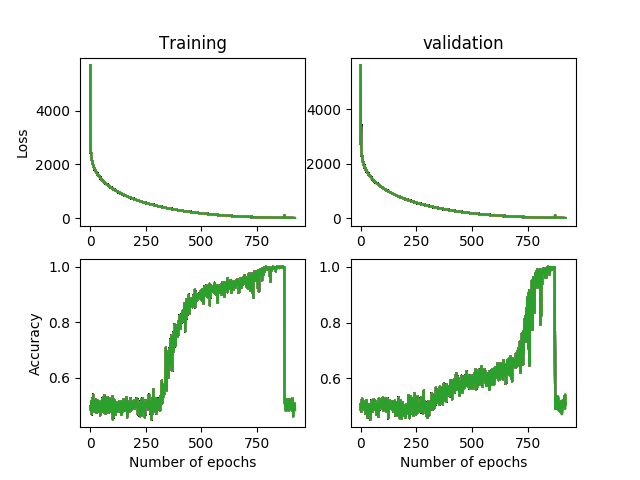
\includegraphics[scale=0.6]{test-batch2-1e-3-80-1e-2-5e-1}
\caption{Batch Size = 80, Learning Rate = 1e-3, Beta = 0.01, Dropout = 0.5}
\end{figure}
\item This run had an optimal validation accuracy of 99.7635 and an optimal test accuracy of 99.7297.  I also tested this multiple times, running the SAME set of hyperparameters, to see what is going on with that weird spike.  Does it keep showing up?  What is going on?  Here are more examples, all run at the same hyperparameters as above:
\begin{figure}[H]
\centering
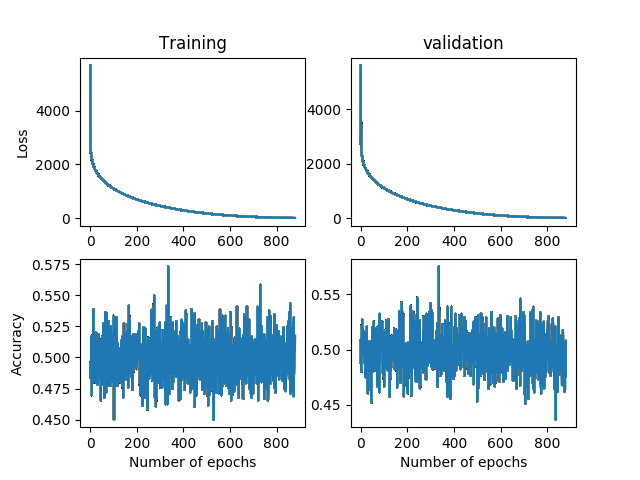
\includegraphics[scale=0.6]{learning-rate-rep1-1e-3-80-1e-2-5e-1}
\caption{Batch Size = 80, Learning Rate = 1e-3, Beta = 0.01, Dropout = 0.5}
\end{figure}
\item This run had an optimal validation accuracy of 47.0608, optimal test accuracy of 47.6689, and final validation accuracy of 49.223, test accuracy of 50.0338 

\begin{figure}[H]
\centering
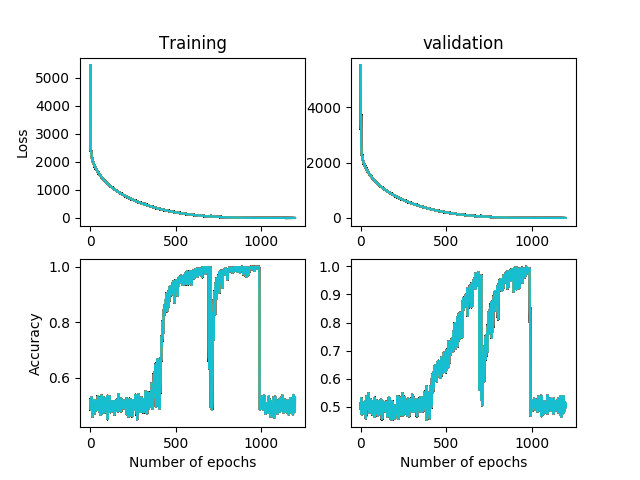
\includegraphics[scale=0.6]{learning-rate-rep2-1e-3-80-1e-2-5e-1}
\caption{Batch Size = 80, Learning Rate = 1e-3, Beta = 0.01, Dropout = 0.5}
\end{figure}
\item This run had an optimal validation accuracy of 99.4595, optimal test accuracy of 99.3243, and final validation accuracy of 50.777, test accuracy of 49.9662. 

\begin{figure}[H]
\centering
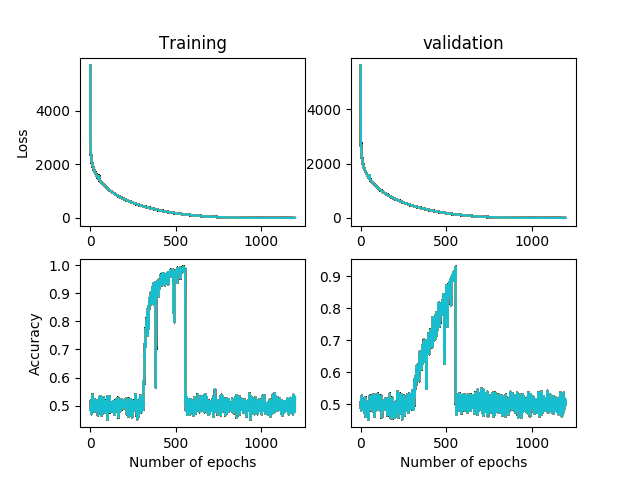
\includegraphics[scale=0.6]{learning-rate-rep3-1e-3-80-1e-2-5e-1}
\caption{Batch Size = 80, Learning Rate = 1e-3, Beta = 0.01, Dropout = 0.5}
\end{figure}
\item This run had an optimal validation accuracy of 992.5, optimal test accuracy of 91.7568, and final validation accuracy of 49.223, test accuracy of 50.0338. 

\begin{figure}[H]
\centering
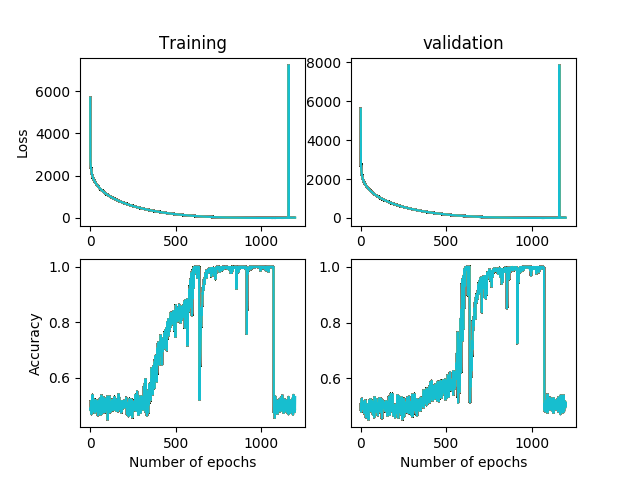
\includegraphics[scale=0.6]{learning-rate-rep4-1e-3-80-1e-2-5e-1}
\caption{Batch Size = 80, Learning Rate = 1e-3, Beta = 0.01, Dropout = 0.5}
\end{figure}
\item This run had an optimal validation accuracy of 99.8987, optimal test accuracy of 99.8649, and final validation accuracy of 50.777, test accuracy of 49.9662. 

\begin{figure}[H]
\centering
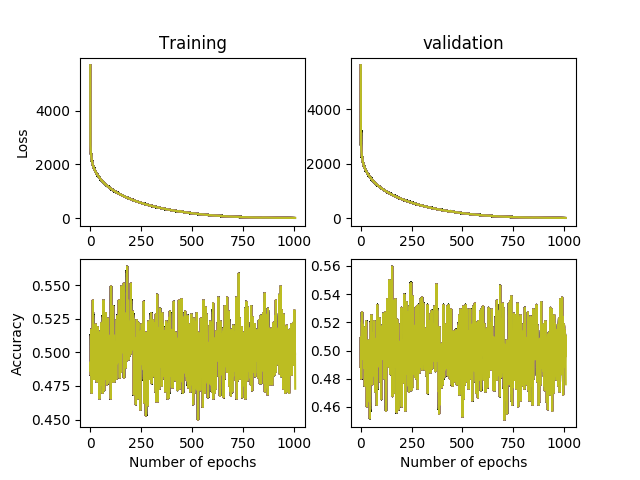
\includegraphics[scale=0.6]{learning-rate-rep5-1e-3-80-1e-2-5e-1}
\caption{Batch Size = 80, Learning Rate = 1e-3, Beta = 0.01, Dropout = 0.5}
\end{figure}
\item This run had an optimal validation accuracy of 55.4054, optimal test accuracy of 54.223, and final validation accuracy of 49,223, test accuracy of 50.0338.

\item The following are images of runs on the dataset that consists of glasses and liquids that are each 12 time steps away from the assumed glass transition temperature of 0.21.  

\begin{figure}[H]
\centering
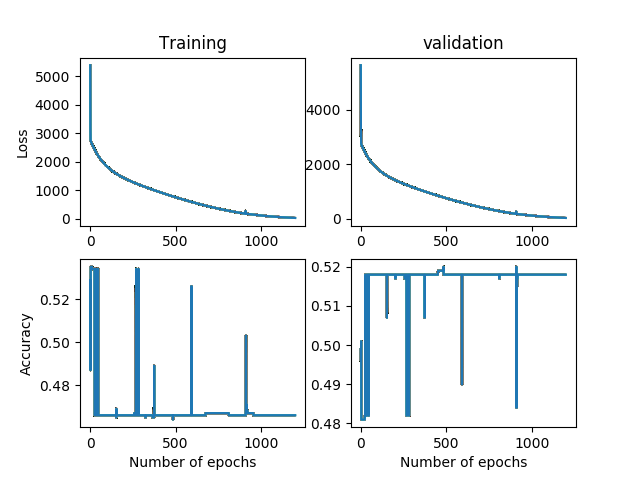
\includegraphics[scale=0.6]{data12-1e-4-100-1e-2-5e-1}
\caption{Batch Size = 100, Learning Rate = 1e-4, Beta = 0.01, Dropout = 0.5}
\end{figure}

\begin{figure}[H]
\centering
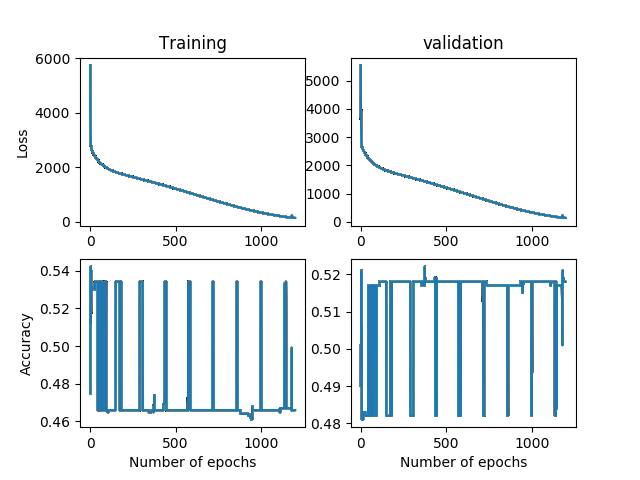
\includegraphics[scale=0.6]{data12-1e-4-10-1e-2-5e-1}
\caption{Batch Size = 10, Learning Rate = 1e-4, Beta = 0.01, Dropout = 0.5}
\end{figure}

\begin{figure}[H]
\centering
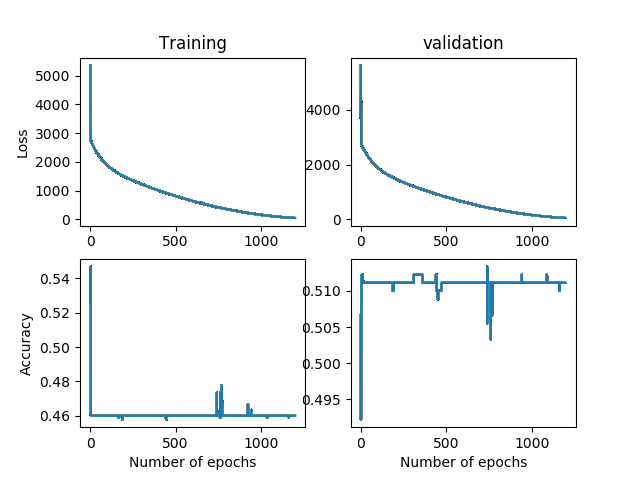
\includegraphics[scale=0.6]{data12-1e-4-150-1e-2-5e-1}
\caption{Batch Size = 150, Learning Rate = 1e-4, Beta = 0.01, Dropout = 0.5}
\end{figure}

\begin{figure}[H]
\centering
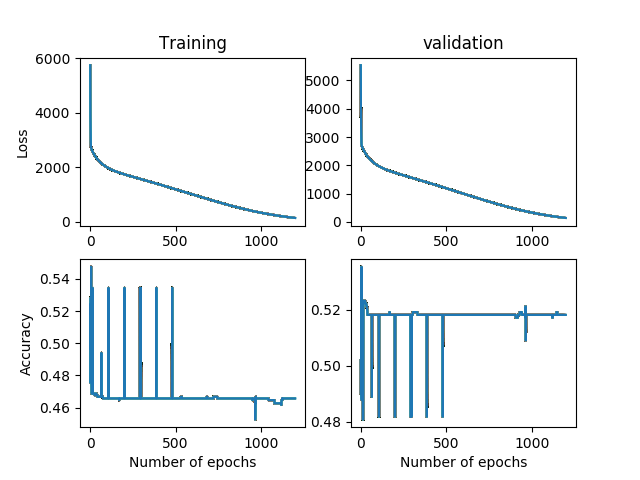
\includegraphics[scale=0.6]{data12-1e-4-15-1e-2-5e-1}
\caption{Batch Size = 15, Learning Rate = 1e-4, Beta = 0.01, Dropout = 0.5}
\end{figure}

\begin{figure}[H]
\centering
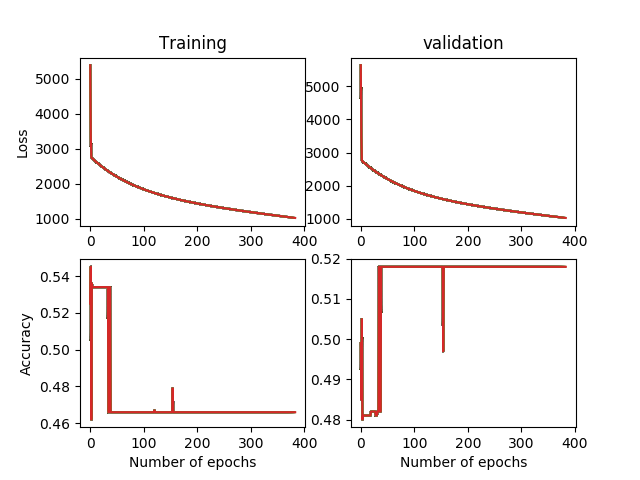
\includegraphics[scale=0.6]{data12-1e-4-200-1e-2-5e-1}
\caption{Batch Size = 200, Learning Rate = 1e-4, Beta = 0.01, Dropout = 0.5}
\end{figure}

\begin{figure}[H]
\centering
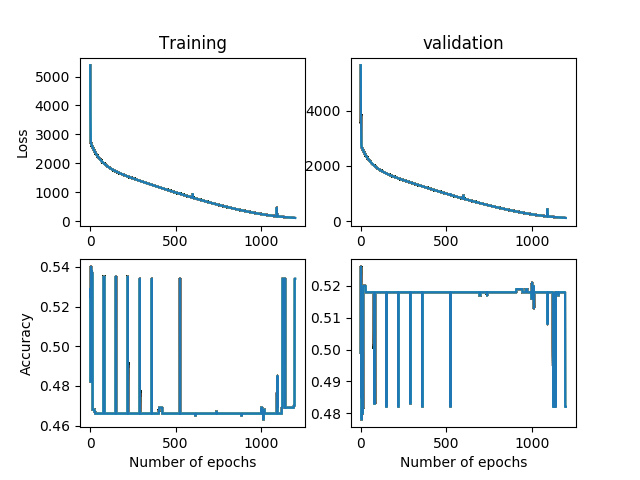
\includegraphics[scale=0.6]{data12-1e-4-20-1e-2-5e-1}
\caption{Batch Size = 20, Learning Rate = 1e-4, Beta = 0.01, Dropout = 0.5}
\end{figure}

\begin{figure}[H]
\centering
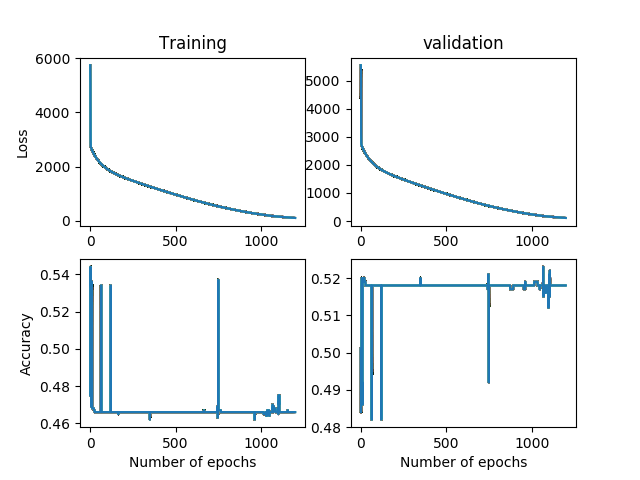
\includegraphics[scale=0.6]{data12-1e-4-25-1e-2-5e-1}
\caption{Batch Size = 25, Learning Rate = 1e-4, Beta = 0.01, Dropout = 0.5}
\end{figure}

\begin{figure}[H]
\centering
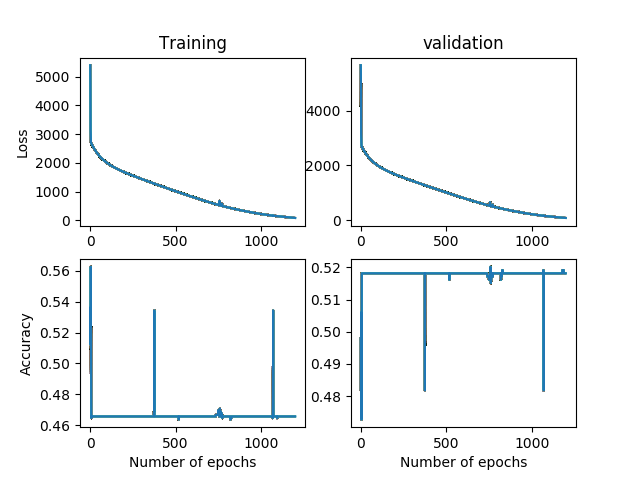
\includegraphics[scale=0.6]{data12-1e-4-30-1e-2-5e-1}
\caption{Batch Size = 30, Learning Rate = 1e-4, Beta = 0.01, Dropout = 0.5}
\end{figure}

\begin{figure}[H]
\centering
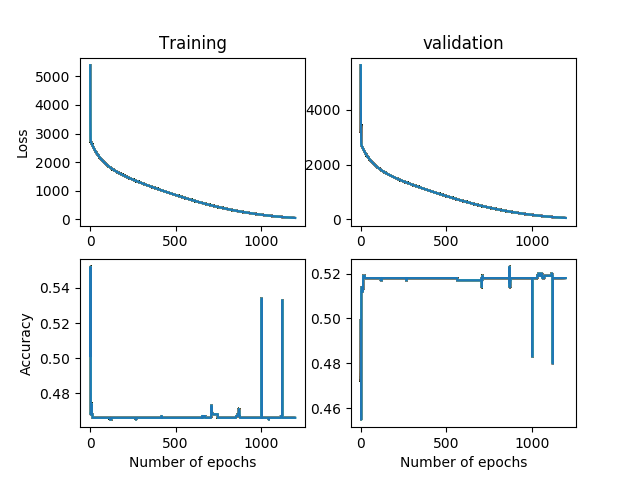
\includegraphics[scale=0.6]{data12-1e-4-50-1e-2-5e-1}
\caption{Batch Size = 50, Learning Rate = 1e-4, Beta = 0.01, Dropout = 0.5}
\end{figure}

\begin{figure}[H]
\centering
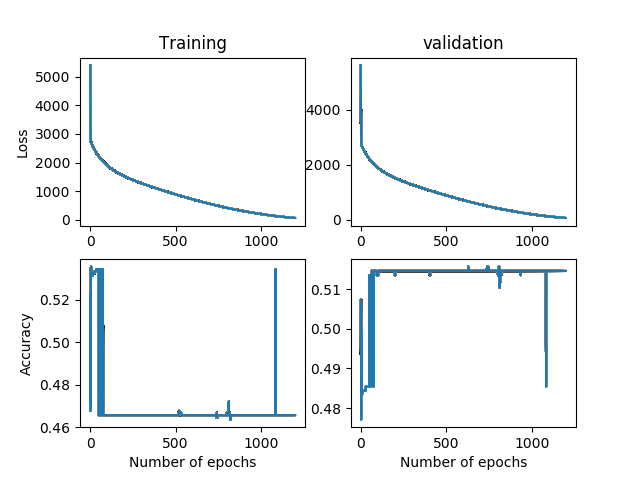
\includegraphics[scale=0.6]{data12-1e-4-80-1e-2-5e-1}
\caption{Batch Size = 80, Learning Rate = 1e-4, Beta = 0.01, Dropout = 0.5}
\end{figure}

\begin{figure}[H]
\centering
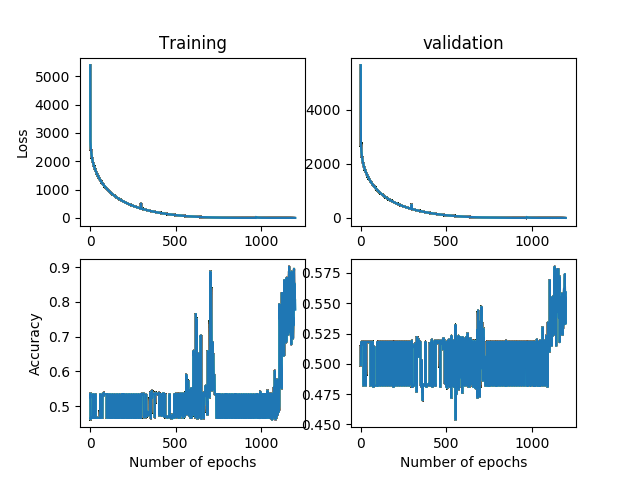
\includegraphics[scale=0.6]{data12-1e-3-100-1e-2-5e-1}
\caption{Batch Size = 100, Learning Rate = 1e-3, Beta = 0.01, Dropout = 0.5}
\end{figure}

\begin{figure}[H]
\centering
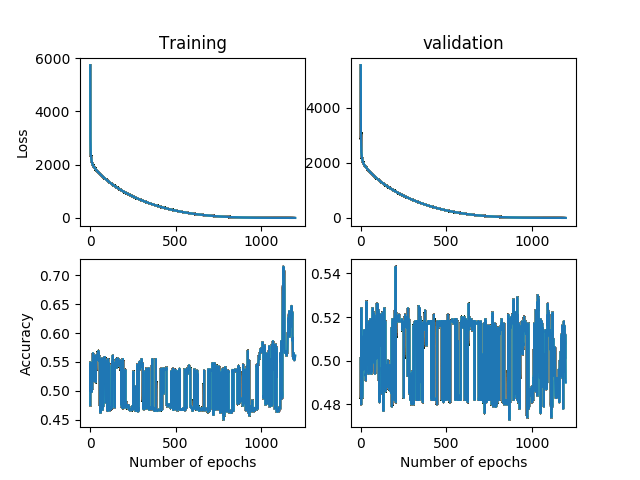
\includegraphics[scale=0.6]{data12-1e-3-10-1e-2-5e-1}
\caption{Batch Size = 10, Learning Rate = 1e-3, Beta = 0.01, Dropout = 0.5}
\end{figure}

\begin{figure}[H]
\centering
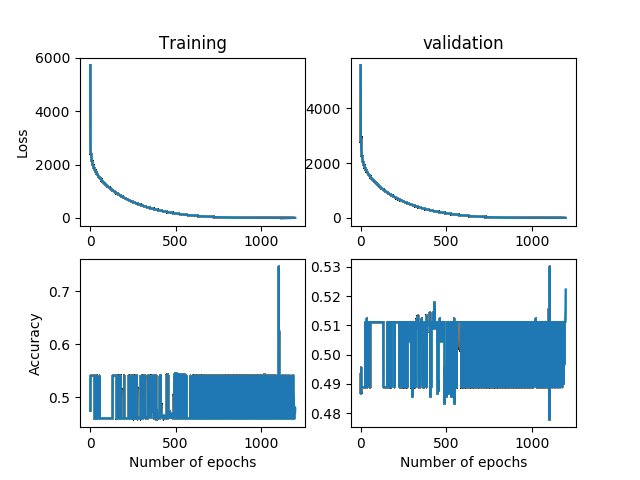
\includegraphics[scale=0.6]{data12-1e-3-150-1e-2-5e-1}
\caption{Batch Size = 150, Learning Rate = 1e-3, Beta = 0.01, Dropout = 0.5}
\end{figure}

\begin{figure}[H]
\centering
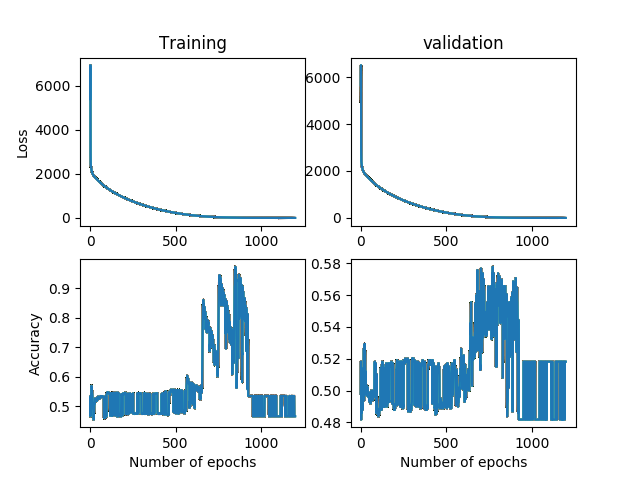
\includegraphics[scale=0.6]{data12-1e-3-15-1e-2-5e-1}
\caption{Batch Size = 15, Learning Rate = 1e-3, Beta = 0.01, Dropout = 0.5}
\end{figure}

\begin{figure}[H]
\centering
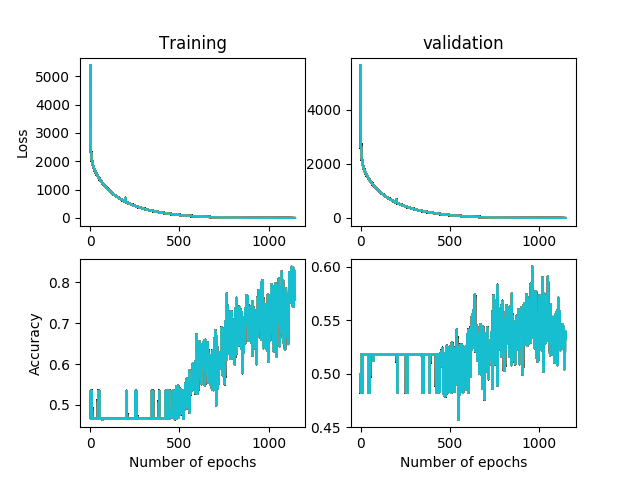
\includegraphics[scale=0.6]{data12-1e-3-200-1e-2-1e-1}
\caption{Batch Size = 200, Learning Rate = 1e-3, Beta = 0.01, Dropout = 0.1}
\end{figure}

\begin{figure}[H]
\centering
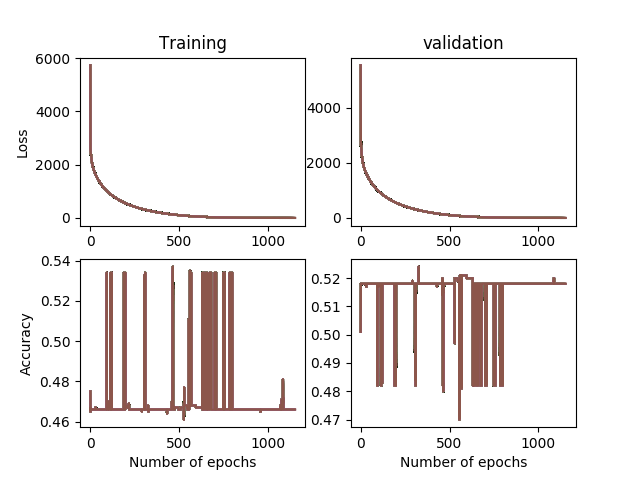
\includegraphics[scale=0.6]{data12-1e-3-200-1e-2-2e-1}
\caption{Batch Size = 200, Learning Rate = 1e-3, Beta = 0.01, Dropout = 0.2}
\end{figure}

\begin{figure}[H]
\centering
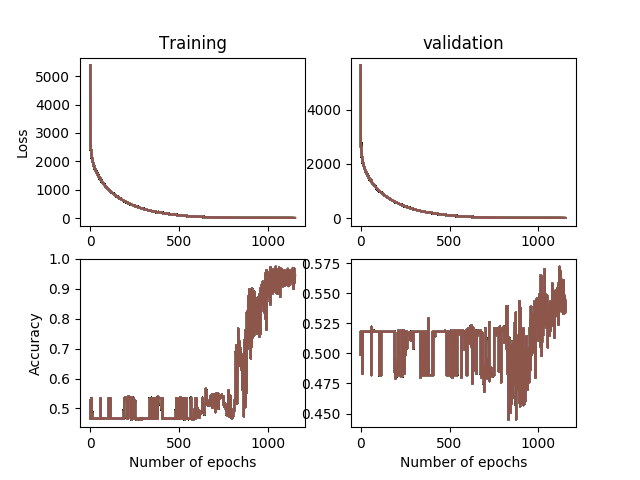
\includegraphics[scale=0.6]{data12-1e-3-200-1e-2-3e-1}
\caption{Batch Size = 200, Learning Rate = 1e-3, Beta = 0.01, Dropout = 0.3}
\end{figure}

\begin{figure}[H]
\centering
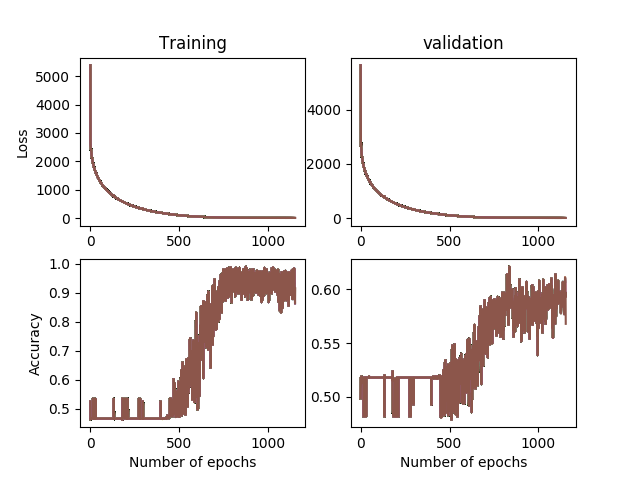
\includegraphics[scale=0.6]{data12-1e-3-200-1e-2-4e-1}
\caption{Batch Size = 200, Learning Rate = 1e-3, Beta = 0.01, Dropout = 0.4}
\end{figure}

\begin{figure}[H]
\centering
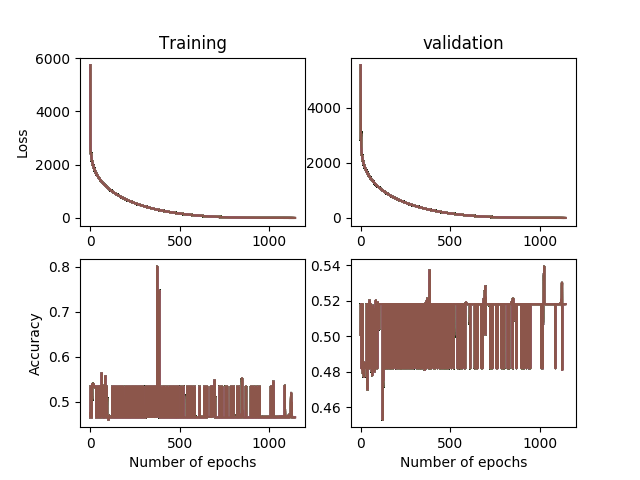
\includegraphics[scale=0.6]{data12-1e-3-200-1e-2-5e-1}
\caption{Batch Size = 200, Learning Rate = 1e-3, Beta = 0.01, Dropout = 0.5}
\end{figure}

\begin{figure}[H]
\centering
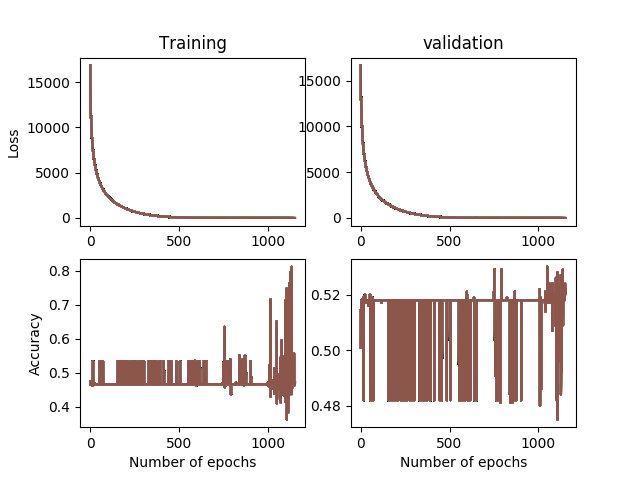
\includegraphics[scale=0.6]{data12-1e-3-200-5e-2-3e-1}
\caption{Batch Size = 200, Learning Rate = 1e-3, Beta = 0.01, Dropout = 0.3}
\end{figure}

\begin{figure}[H]
\centering
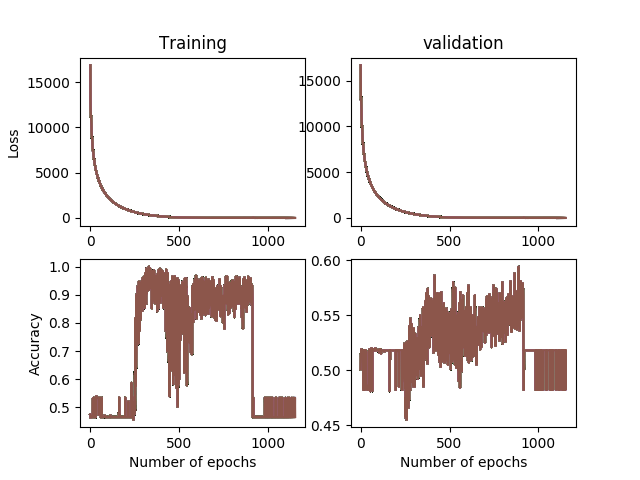
\includegraphics[scale=0.6]{data12-1e-3-200-5e-2-4e-1}
\caption{Batch Size = 200, Learning Rate = 1e-3, Beta = 0.01, Dropout = 0.4}
\end{figure}

\begin{figure}[H]
\centering
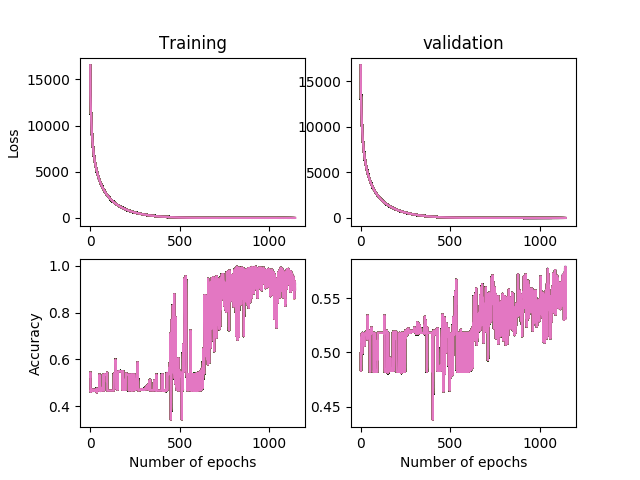
\includegraphics[scale=0.6]{data12-1e-3-200-5e-2-5e-1}
\caption{Batch Size = 200, Learning Rate = 1e-3, Beta = 0.01, Dropout = 0.4}
\end{figure}

\begin{figure}[H]
\centering
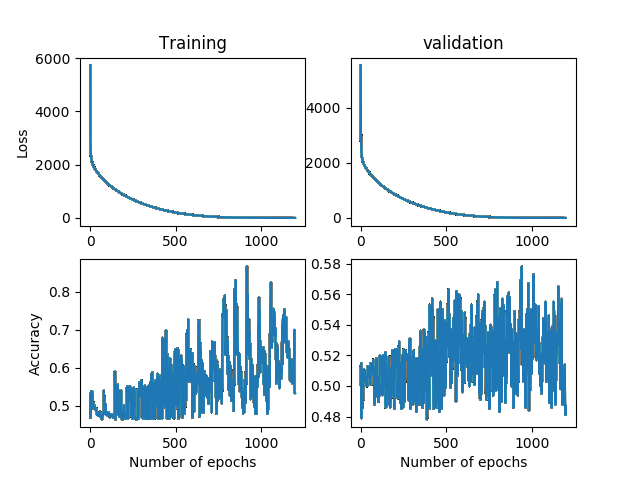
\includegraphics[scale=0.6]{data12-1e-3-20-1e-2-5e-1}
\caption{Batch Size = 20, Learning Rate = 1e-3, Beta = 0.01, Dropout = 0.5}
\end{figure}

\begin{figure}[H]
\centering
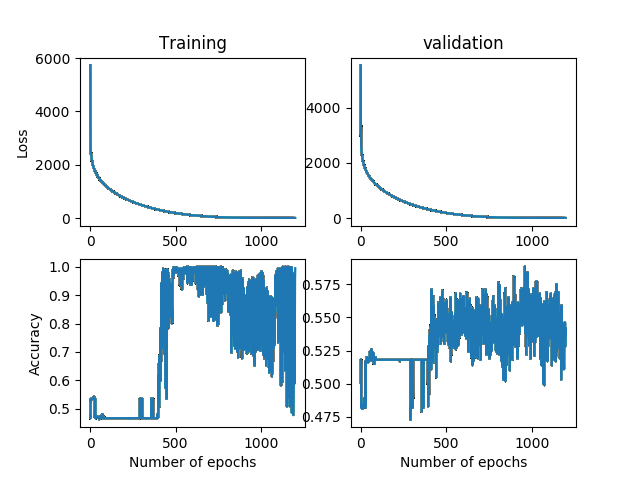
\includegraphics[scale=0.6]{data12-1e-3-250-1e-2-5e-1}
\caption{Batch Size = 250, Learning Rate = 1e-3, Beta = 0.01, Dropout = 0.5}
\end{figure}

\begin{figure}[H]
\centering
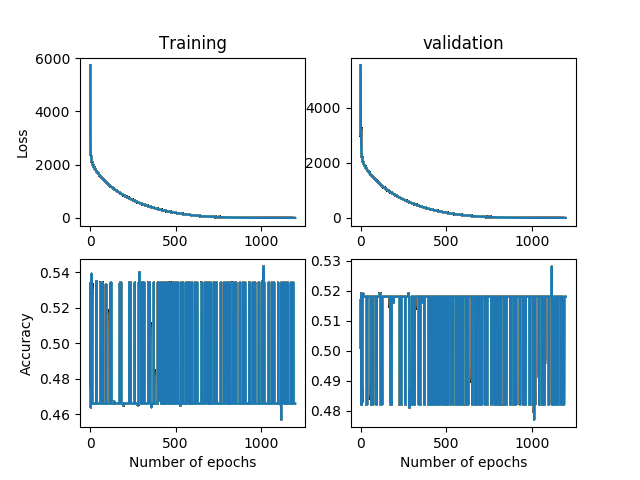
\includegraphics[scale=0.6]{data12-1e-3-25-1e-2-5e-1}
\caption{Batch Size = 25, Learning Rate = 1e-3, Beta = 0.01, Dropout = 0.5}
\end{figure}

\begin{figure}[H]
\centering
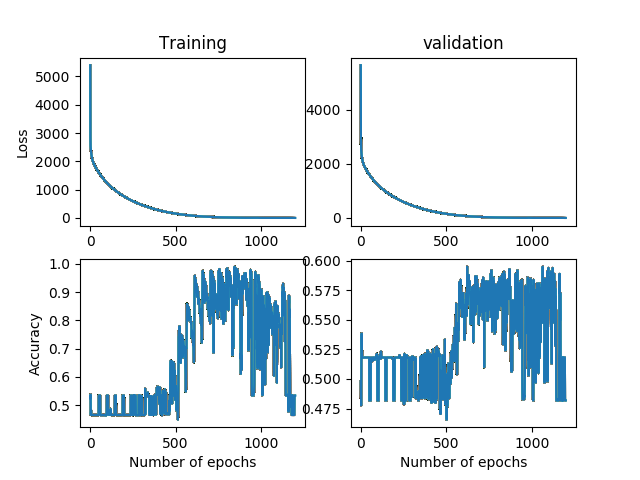
\includegraphics[scale=0.6]{data12-1e-3-30-1e-2-5e-1}
\caption{Batch Size = 30, Learning Rate = 1e-3, Beta = 0.01, Dropout = 0.5}
\end{figure}

\begin{figure}[H]
\centering
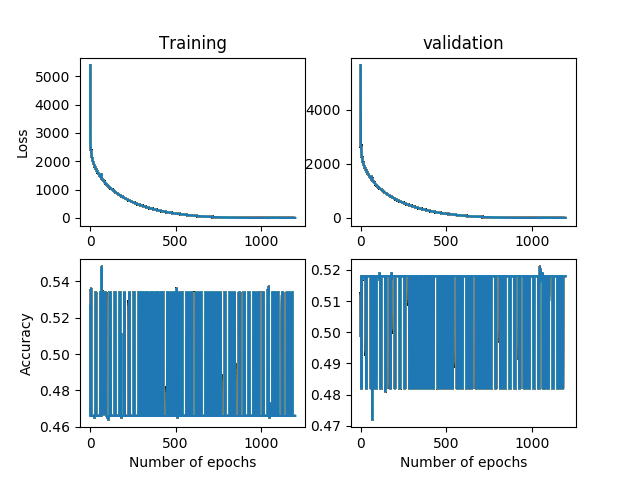
\includegraphics[scale=0.6]{data12-1e-3-50-1e-2-5e-1}
\caption{Batch Size = 50, Learning Rate = 1e-3, Beta = 0.01, Dropout = 0.5}
\end{figure}

\item Visualizations.  
\begin{figure}[H]
\centering
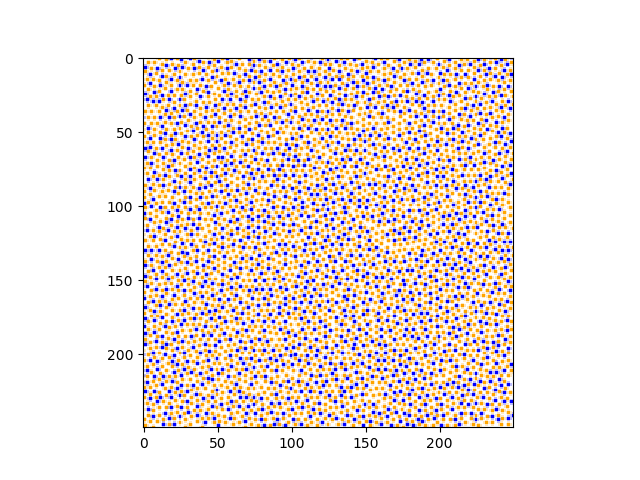
\includegraphics[scale=0.6]{glass_original}
\caption{Glass original}
\end{figure}

\begin{figure}[H]
\centering
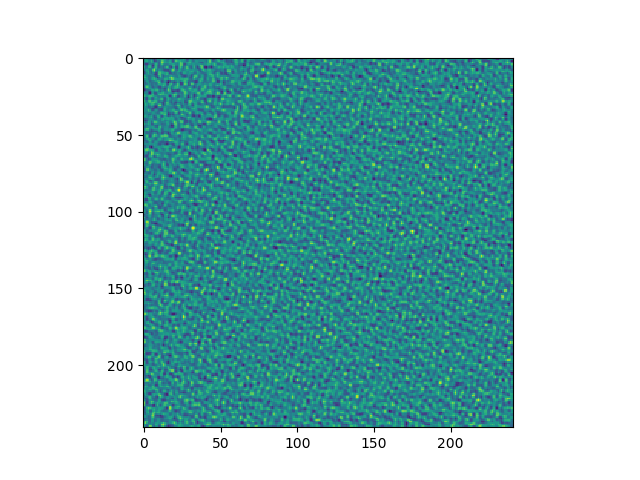
\includegraphics[scale=0.6]{glass_channel_1}
\caption{Glass channel 1}
\end{figure}

\begin{figure}[H]
\centering
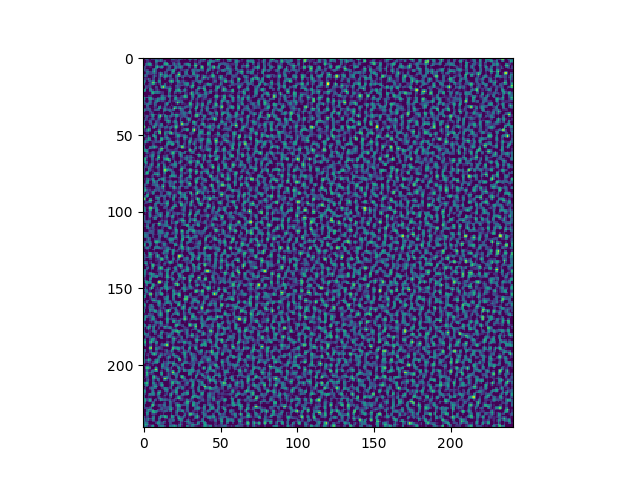
\includegraphics[scale=0.6]{glass_channel_2}
\caption{Glass channel 2}
\end{figure}

\begin{figure}[H]
\centering
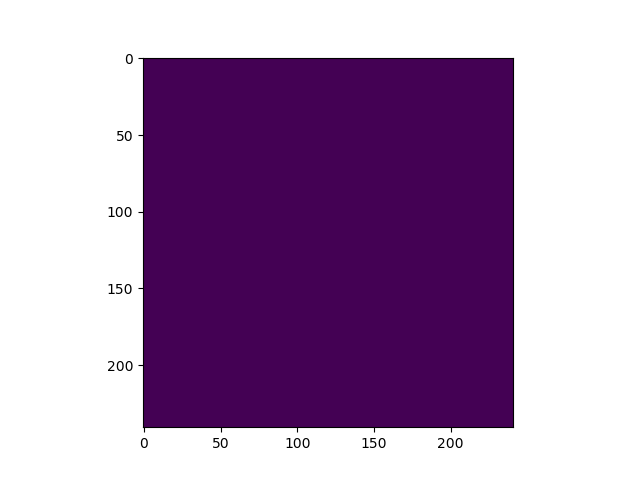
\includegraphics[scale=0.6]{glass_channel_3}
\caption{Glass channel 3}
\end{figure}

\begin{figure}[H]
\centering
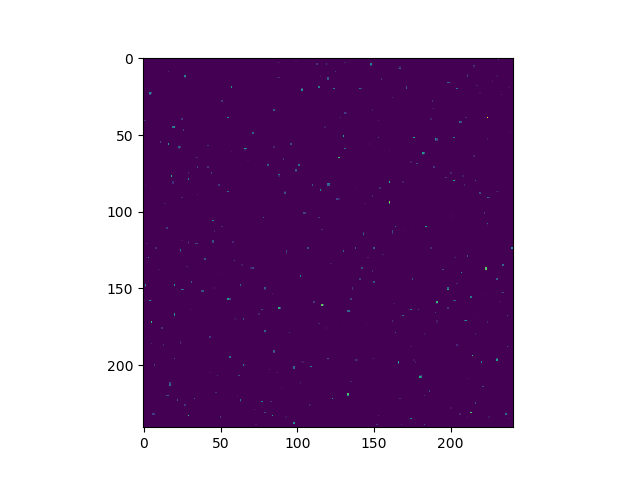
\includegraphics[scale=0.6]{glass_channel_4}
\caption{Glass channel 4}
\end{figure}

\begin{figure}[H]
\centering
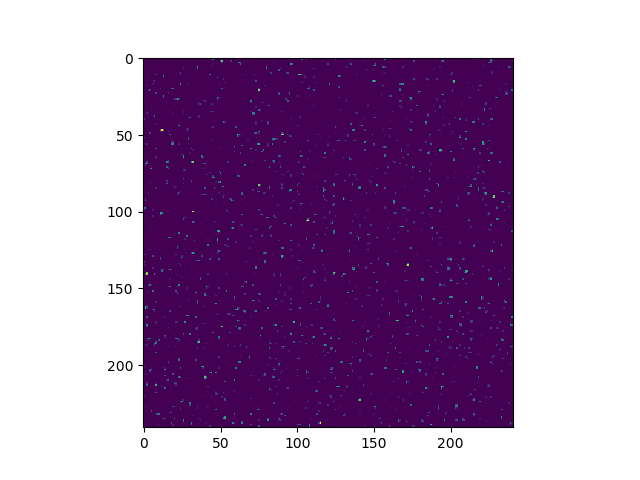
\includegraphics[scale=0.6]{glass_channel_5}
\caption{Glass channel 5}
\end{figure}

\begin{figure}[H]
\centering
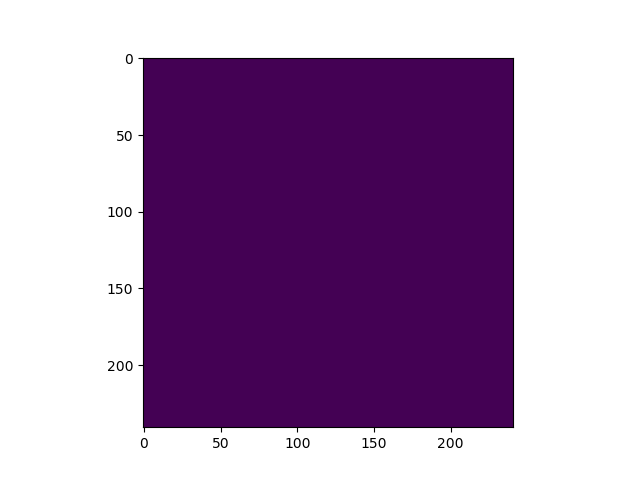
\includegraphics[scale=0.6]{glass_channel_6}
\caption{Glass channel 6}
\end{figure}

\begin{figure}[H]
\centering
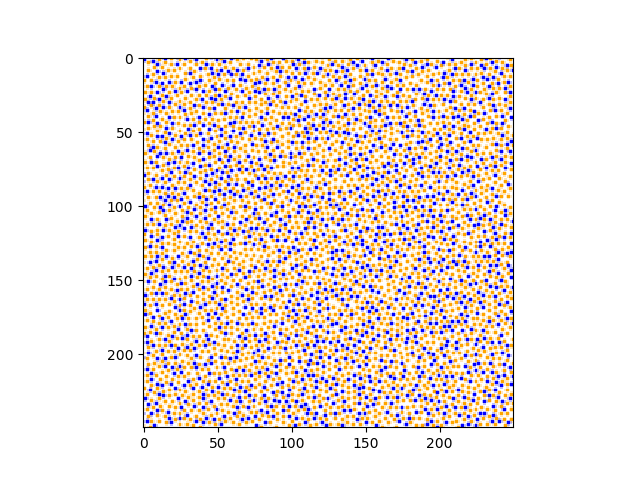
\includegraphics[scale=0.6]{liquid_original}
\caption{Liquid original}
\end{figure}

\begin{figure}[H]
\centering
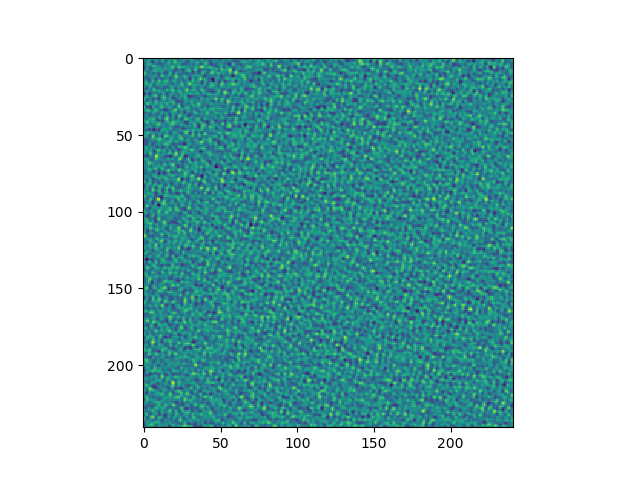
\includegraphics[scale=0.6]{liquid_channel_1}
\caption{Liquid channel 1}
\end{figure}

\begin{figure}[H]
\centering
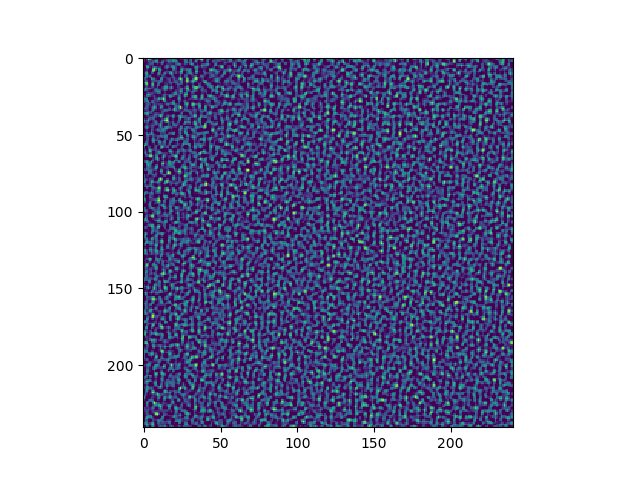
\includegraphics[scale=0.6]{liquid_channel_2}
\caption{Liquid channel 2}
\end{figure}

\begin{figure}[H]
\centering
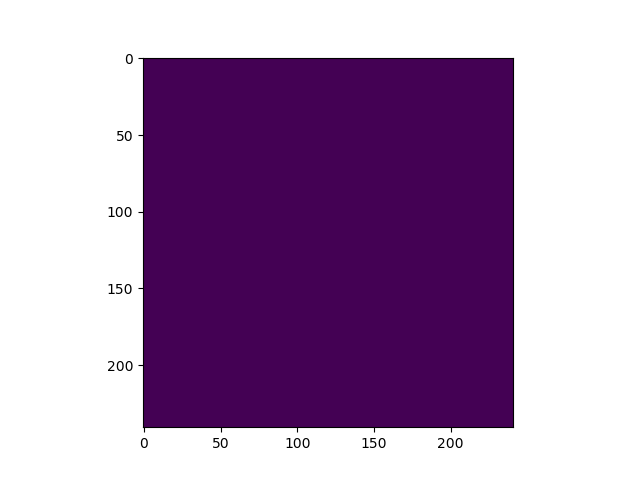
\includegraphics[scale=0.6]{liquid_channel_3}
\caption{Liquid channel 3}
\end{figure}

\begin{figure}[H]
\centering
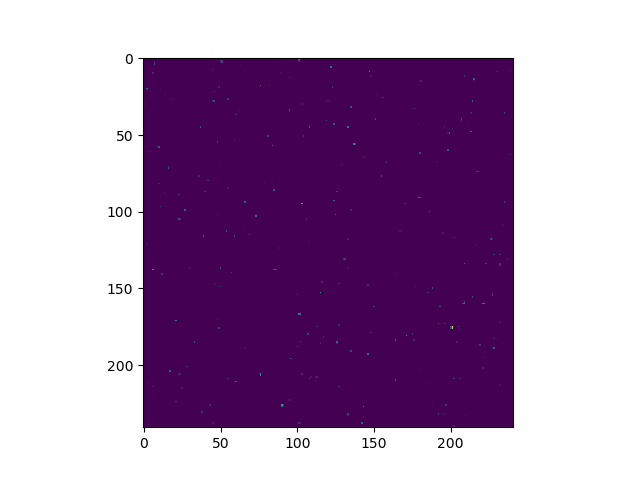
\includegraphics[scale=0.6]{liquid_channel_4}
\caption{Liquid channel 4}
\end{figure}

\begin{figure}[H]
\centering
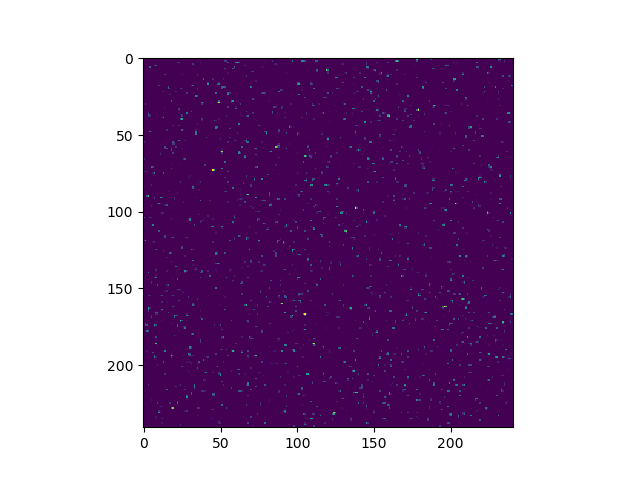
\includegraphics[scale=0.6]{liquid_channel_5}
\caption{Liquid channel 5}
\end{figure}

\begin{figure}[H]
\centering
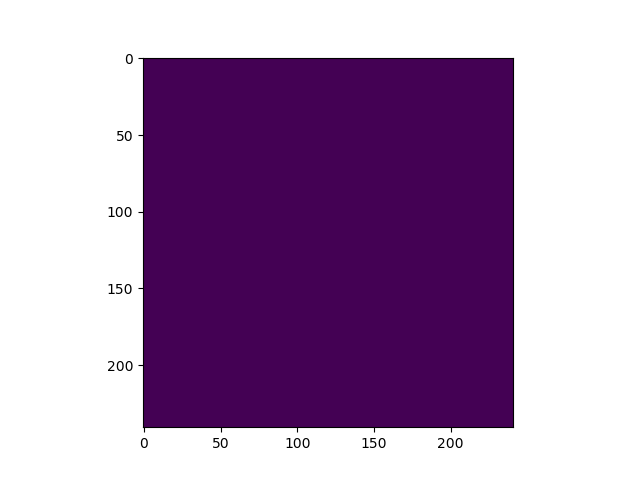
\includegraphics[scale=0.6]{liquid_channel_6}
\caption{Liquid channel 6}
\end{figure}

\end{enumerate}

\section{12/13/2017}
\begin{enumerate}
\item Updated python scripts and merged with GitHub - the recent additions include streamlining the learning rate schedule and data augmentation options.  The following is for a standard run on the original endpoint data:

\begin{figure}[H]
\centering
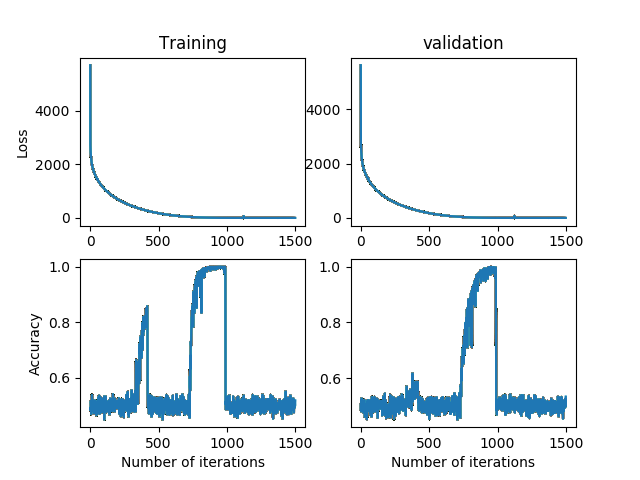
\includegraphics[scale=0.6]{test-1e-3-1e-3-550-80-1e-2-5e-1}
\caption{Initial Learning Rate = 1e-3, Final Learning Rate = 1e-3, Schedule Length = 550 iterations, Batch Size = 80, L2 beta = 0.01, Dropout = 0.5}
\end{figure}

\item I then, twice, set the final learning rate to be smaller, at 1e-4:

\begin{figure}[H]
\centering
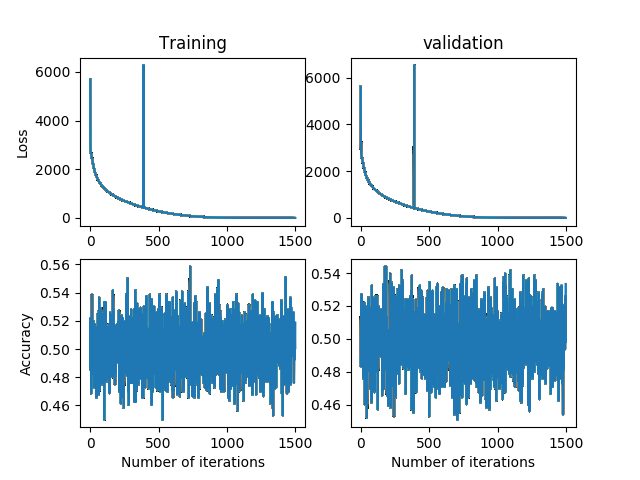
\includegraphics[scale=0.6]{test-1e-4-1e-3-550-80-1e-2-5e-1}
\caption{Initial Learning Rate = 1e-3, Final Learning Rate = 1e-3, Schedule Length = 550 iterations, Batch Size = 80, L2 beta = 0.01, Dropout = 0.5}
\end{figure}

\begin{figure}[H]
\centering
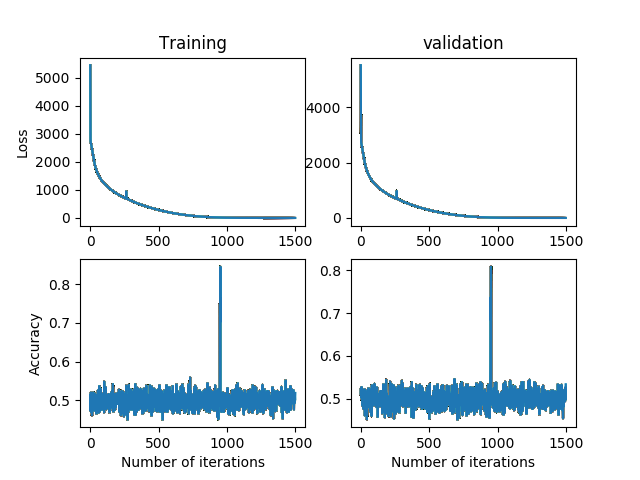
\includegraphics[scale=0.6]{test2-1e-4-1e-3-550-80-1e-2-5e-1}
\caption{Initial Learning Rate = 1e-3, Final Learning Rate = 1e-3, Schedule Length = 550 iterations, Batch Size = 80, L2 beta = 0.01, Dropout = 0.5}
\end{figure}

\item What is going on here?  It seems as though setting the learning rate a magnitude lower really screws things up...
\item Note: one iteration goes through 10 batches, so if the batch size is 80, then one iteration goes through 800 examples.  The training set is 70 percent of the total 20,000 images, so the training set is 14,000 images.  Thus, one epoch is 17.5 iterations, or approximately 18 iterations.  That means that 1500 iterations is about 83 epochs.  Question: how many epochs is typically needed for a binary classification problem?  And how long does this typically take?
\item I also tested the usual hyperparameters on the original endpoint data and turned on the data augmentation, to see if there would be any issues.  I got the following training runs:

\begin{figure}[H]
\centering
\includegraphics[scale=0.6]{data_aug}
\caption{Initial Learning Rate = NA, Final Learning Rate = 1e-3, Schedule Length = NA, Batch Size = 80, L2 beta = 0.01, Dropout = 0.5}
\end{figure}

\begin{figure}[H]
\centering
\includegraphics[scale=0.6]{data_aug2}
\caption{Initial Learning Rate = NA, Final Learning Rate = 1e-3, Schedule Length = NA, Batch Size = 80, L2 beta = 0.01, Dropout = 0.5}
\end{figure}

\begin{figure}[H]
\centering
\includegraphics[scale=0.6]{data_aug3}
\caption{Initial Learning Rate = NA, Final Learning Rate = 1e-3, Schedule Length = NA, Batch Size = 80, L2 beta = 0.01, Dropout = 0.5}
\end{figure}

\begin{figure}[H]
\centering
\includegraphics[scale=0.6]{data_aug4}
\caption{Initial Learning Rate = NA, Final Learning Rate = 1e-3, Schedule Length = NA, Batch Size = 80, L2 beta = 0.01, Dropout = 0.5}
\end{figure}

\begin{figure}[H]
\centering
\includegraphics[scale=0.6]{data_aug5}
\caption{Initial Learning Rate = NA, Final Learning Rate = 1e-3, Schedule Length = NA, Batch Size = 80, L2 beta = 0.01, Dropout = 0.5}
\end{figure}

\item I should double check that the dataset augmentation is actually working.  
\end{enumerate}
\section{12/22/2017}
\begin{enumerate}
\item I am now going to run a series of training runs that will explore the relationship between the learning rate schedule and accuracy.  First, let's try the threshold idea.  Then, we will try the standard exponential decay idea.  Let's try the following.  When the accuracy gets to 90 percent, let's decrease the learning rate by an order of magnitude.  Let's just run that simple test, say, 8 times, and see what happens!

\item Initial learning rate = , Final learning rate = ,   
\end{enumerate}
\section{12/24/2017}
\begin{enumerate}
\item We ran a series of training runs that used a learning rate threshold.  The learning rate starts at the initial learning rate.  The learning rate changes to the final learning rate whenever the validation accuracy is above 90 percent.  This allows the learning rate to go back to the initial learning rate if the accuracy drops below 90 percent.  Here are plots showing six tests.  These plots demonstrate that the sharp drops in accuracy were, indeed, the result of a learning rate that was too large towards the end of training, since there are no sharp drops in accuracy here:

\begin{figure}[H]
\centering
\includegraphics[scale=0.6]{threshold-test-1e-3-1e-4-1}
\caption{Initial Learning Rate = 1e-3, Final Learning Rate = 1e-4, Schedule Length = NA, Batch Size = 80, L2 beta = 0.01, Dropout = 0.5}
\end{figure}

\begin{figure}[H]
\centering
\includegraphics[scale=0.6]{threshold-test-1e-3-1e-4-2}
\caption{Initial Learning Rate = 1e-3, Final Learning Rate = 1e-4, Schedule Length = NA, Batch Size = 80, L2 beta = 0.01, Dropout = 0.5}
\end{figure}

\begin{figure}[H]
\centering
\includegraphics[scale=0.6]{threshold-test-1e-3-1e-4-3}
\caption{Initial Learning Rate = 1e-3, Final Learning Rate = 1e-4, Schedule Length = NA, Batch Size = 80, L2 beta = 0.01, Dropout = 0.5}
\end{figure}

\begin{figure}[H]
\centering
\includegraphics[scale=0.6]{threshold-test-1e-3-1e-5-1}
\caption{Initial Learning Rate = 1e-3, Final Learning Rate = 1e-4, Schedule Length = NA, Batch Size = 80, L2 beta = 0.01, Dropout = 0.5}
\end{figure}

\begin{figure}[H]
\centering
\includegraphics[scale=0.6]{threshold-test-1e-3-1e-5-2}
\caption{Initial Learning Rate = 1e-3, Final Learning Rate = 1e-4, Schedule Length = NA, Batch Size = 80, L2 beta = 0.01, Dropout = 0.5}
\end{figure}

\begin{figure}[H]
\centering
\includegraphics[scale=0.6]{threshold-test-1e-3-1e-5-3}
\caption{Initial Learning Rate = 1e-3, Final Learning Rate = 1e-4, Schedule Length = NA, Batch Size = 80, L2 beta = 0.01, Dropout = 0.5}
\end{figure}

\end{enumerate}

\subsection{12/29/2017}
\begin{enumerate}
\item Ran another series of runs that used a similar learning rate threshold just to check that my GitHub had been updated appropriately.  This time used only 1e-3 to 1e-4.  In one example, the accuracy crashed.  Perhaps evidences that smaller learning rates are needed closer to the minimum.  For the sake of completeness, these extra runs are reported below:  

\begin{figure}[H]
\centering
\includegraphics[scale=0.6]{Commit-test-1}
\caption{Initial Learning Rate = 1e-3, Final Learning Rate = 1e-4, Schedule Length = NA, Batch Size = 80, L2 beta = 0.01, Dropout = 0.5}
\end{figure}

\begin{figure}[H]
\centering
\includegraphics[scale=0.6]{Commit-test-2}
\caption{Initial Learning Rate = 1e-3, Final Learning Rate = 1e-4, Schedule Length = NA, Batch Size = 80, L2 beta = 0.01, Dropout = 0.5}
\end{figure}

\begin{figure}[H]
\centering
\includegraphics[scale=0.6]{Commit-test-3}
\caption{Initial Learning Rate = 1e-3, Final Learning Rate = 1e-4, Schedule Length = NA, Batch Size = 80, L2 beta = 0.01, Dropout = 0.5}
\end{figure}

\begin{figure}[H]
\centering
\includegraphics[scale=0.6]{Commit-test-4}
\caption{Initial Learning Rate = 1e-3, Final Learning Rate = 1e-4, Schedule Length = NA, Batch Size = 80, L2 beta = 0.01, Dropout = 0.5}
\end{figure}

\begin{figure}[H]
\centering
\includegraphics[scale=0.6]{Commit-test-5}
\caption{Initial Learning Rate = 1e-3, Final Learning Rate = 1e-4, Schedule Length = NA, Batch Size = 80, L2 beta = 0.01, Dropout = 0.5}
\end{figure}

\begin{figure}[H]
\centering
\includegraphics[scale=0.6]{Commit-test-6}
\caption{Initial Learning Rate = 1e-3, Final Learning Rate = 1e-4, Schedule Length = NA, Batch Size = 80, L2 beta = 0.01, Dropout = 0.5}
\end{figure}

\begin{figure}[H]
\centering
\includegraphics[scale=0.6]{Commit-test-7}
\caption{Initial Learning Rate = 1e-3, Final Learning Rate = 1e-4, Schedule Length = NA, Batch Size = 80, L2 beta = 0.01, Dropout = 0.5}
\end{figure}


\end{enumerate}

\subsection{12/30/2017}
\begin{enumerate}
\item Tested the data augmentation scheme manually.  Printed out a series of images and their respective augmented versions that are given when generator.next is invoked, respectively with the data aug option set to false and with the data aug option set to true.  

\end{enumerate}

\subsection{1/1/2018}
\begin{enumerate}
\item Added main\_glassliquid\_restart.py, a file that can run training starting from a previous saved model.  Tested it.  Now, let's try to train again on the dataset that consists of glasses and liquids that are each 12 time steps away from the assumed glass transition temperature of 0.21.  Previously, the best parameters were batch size 200, learning rate 1e-3, beta 0.01, dropout 0.4.  Now, we are going to do a series of simulations using the same parameters, except, first, we are going to include dataset augmentation, and second, we are going to run the simluation at least twice as long.  Then, once we get a sense for how these train, we will add in a learning rate threshold step, or even multiple threshold steps if necessary!     

\end{enumerate}

\subsection{1/4/2018}
\begin{enumerate}
\item Realized that I had run on the original endpoint data.  So, copied over the folder called "data\_12steps" into the current machine-learning-glasses directory, removed the current metadata folder, and created a new metadata folder with this data.  Then, set up new training runs again.      

\end{enumerate}

\section{1/9/2018}
\begin{enumerate}
\item Collected data from the above-mentioned simulations.  The training curves are as follows:

\begin{figure}[H]
\centering
\includegraphics[scale=0.6]{data12_version1_step0}
\caption{Version 1: Initial Learning Rate = 1e-3, Final Learning Rate = 1e-4, Schedule Length = NA, Batch Size = 80, L2 beta = 0.01, Dropout = 0.4, data aug = true}
\end{figure}

\begin{figure}[H]
\centering
\includegraphics[scale=0.6]{data12_version2_step0}
\caption{Version 2: Initial Learning Rate = 1e-3, Final Learning Rate = 1e-4, Schedule Length = NA, Batch Size = 80, L2 beta = 0.01, Dropout = 0.4, data aug = true}
\end{figure}

\begin{figure}[H]
\centering
\includegraphics[scale=0.6]{data12_version3_step0}
\caption{Version 3: Initial Learning Rate = 1e-3, Final Learning Rate = 1e-4, Schedule Length = NA, Batch Size = 80, L2 beta = 0.01, Dropout = 0.4, data aug = true}
\end{figure}

\begin{figure}[H]
\centering
\includegraphics[scale=0.6]{data12_version4_step0}
\caption{Version 4: Initial Learning Rate = 1e-3, Final Learning Rate = 1e-4, Schedule Length = NA, Batch Size = 80, L2 beta = 0.01, Dropout = 0.4, data aug = true}
\end{figure}

\begin{figure}[H]
\centering
\includegraphics[scale=0.6]{data12_version5_step0}
\caption{Version 5: Initial Learning Rate = 1e-3, Final Learning Rate = 1e-4, Schedule Length = NA, Batch Size = 80, L2 beta = 0.01, Dropout = 0.4, data aug = true}
\end{figure}

\begin{figure}[H]
\centering
\includegraphics[scale=0.6]{data12_version6_step0}
\caption{Version 6: Initial Learning Rate = 1e-3, Final Learning Rate = 1e-4, Schedule Length = NA, Batch Size = 80, L2 beta = 0.01, Dropout = 0.4, data aug = true}
\end{figure}

\item The problem is that my allotted time (36 hours) was not enough, so the simulations terminated early.  My program, however, was only set to save the current model at the end of the iterations.  So, the current model was not saved, only the best model was saved.  So, I went back into the main code and changed it so that the current model is updated and saved at every iteration, in addition to the best model being updated when necessary.  I also included restart capability into the main code (using parsing options), so that there is not a separate restart file.  

\item I am now running 7 new simulations.  The first is just a re-do of version1 step 0.  The others take version5 step 0 and start from the saved best model as a starting point, using the new restart capabilities of the main code.  The first two simulations from this starting point (version5 step2 and version5 step2 trial2) use the original parameters.  The next two (version5 step2 trial3 and version5 step2 trial4 use eta\_initial=1e-4 and eta\_final=1e-5), and the final two (version5 step2 trial5 and version5 step2 trial6) use eta\_intial=1e-5 and eta\_final=1e-6.  We will see how these 7 new runs turn out.  
\end{enumerate}

\subsection{1/14/2018}
\begin{enumerate}
\item Here is the result for the continuations from Version 5 step 0, i.e. Version 5 step 1 trials 1 through 6.  

\begin{figure}[H]
\centering
\includegraphics[scale=0.6]{data12_version5_step1}
\caption{Version 5 step 1 trial 1: Initial Learning Rate = 1e-3, Final Learning Rate = 1e-4, Schedule Length = NA, Batch Size = 80, L2 beta = 0.01, Dropout = 0.4, data aug = true}
\end{figure}

\begin{figure}[H]
\centering
\includegraphics[scale=0.6]{data12_version5_step1_trial2}
\caption{Version 5 step 1 trial 2: Initial Learning Rate = 1e-3, Final Learning Rate = 1e-4, Schedule Length = NA, Batch Size = 80, L2 beta = 0.01, Dropout = 0.4, data aug = true}
\end{figure}

\begin{figure}[H]
\centering
\includegraphics[scale=0.6]{data12_version5_step1_trial3}
\caption{Version 5 step 1 trial 3: Initial Learning Rate = 1e-4, Final Learning Rate = 1e-5, Schedule Length = NA, Batch Size = 80, L2 beta = 0.01, Dropout = 0.4, data aug = true}
\end{figure}

\begin{figure}[H]
\centering
\includegraphics[scale=0.6]{data12_version5_step1_trial4}
\caption{Version 5 step 1 trial 4: Initial Learning Rate = 1e-4, Final Learning Rate = 1e-5, Schedule Length = NA, Batch Size = 80, L2 beta = 0.01, Dropout = 0.4, data aug = true}
\end{figure}

\begin{figure}[H]
\centering
\includegraphics[scale=0.6]{data12_version5_step1_trial5}
\caption{Version 5 step 1 trial 5: Initial Learning Rate = 1e-5, Final Learning Rate = 1e-6, Schedule Length = NA, Batch Size = 80, L2 beta = 0.01, Dropout = 0.4, data aug = true}
\end{figure}

\begin{figure}[H]
\centering
\includegraphics[scale=0.6]{data12_version5_step1_trial6}
\caption{Version 5 step 1 trial 6: Initial Learning Rate = 1e-5, Final Learning Rate = 1e-6, Schedule Length = NA, Batch Size = 80, L2 beta = 0.01, Dropout = 0.4, data aug = true}
\end{figure}

\item I am now going to generate new data that is farther away from the assumed glass transition temperature of $T_g = 0.21$.  Based on cooling.dat file in the folder N2e7/0, which is the first of 10,000 simulations, this temperature is at the 184th line of the file (0.21575), which is the 183rd time listed.  There are 200 times listed in cooling.dat, each one separated by a time length of 100,000 time steps.  This is because the total simulation is 2e7, or 20 million.  In the folder /project/depablo/kswanson/2017, I open the file make\_images\_kirk.sh and change the liquid generation number to 500000 and keep the glass generation number at 20000000.   



\end{enumerate}

\subsection{1/15/2018}
\begin{enumerate}
\item After generating the new datapoint, I create a folder called data\_liquid5 and transfer it to the git repo.  Now, I delete the current metadata folder and create a new metadata folder that contains the data\_liquid5 in it.  
\item V1-S1 has hyperparameters:  Initial Learning Rate = 1e-3, Final Learning Rate = 1e-4, eta threshold = 0.90, Batch Size = 10, L2 beta = 0.01, Dropout = 0.5, data aug = true.
\item V2-S1 has hyperparameters:  Initial Learning Rate = 1e-3, Final Learning Rate = 1e-4, eta threshold = 0.90, Batch Size = 10, L2 beta = 0.01, Dropout = 0.5, data aug = true.    
\item V3-S1 has hyperparameters:  Initial Learning Rate = 1e-3, Final Learning Rate = 1e-4, eta threshold = 0.90, Batch Size = 20, L2 beta = 0.01, Dropout = 0.5, data aug = true.  
\item V4-S1 has hyperparameters:  Initial Learning Rate = 1e-3, Final Learning Rate = 1e-4, eta threshold = 0.90, Batch Size = 20, L2 beta = 0.01, Dropout = 0.5, data aug = true.  
\item V5-S1 has hyperparameters:  Initial Learning Rate = 1e-3, Final Learning Rate = 1e-4, eta threshold = 0.90, Batch Size = 30, L2 beta = 0.01, Dropout = 0.5, data aug = true. 
\item V6-S1 has hyperparameters:  Initial Learning Rate = 1e-3, Final Learning Rate = 1e-4, eta threshold = 0.90, Batch Size = 30, L2 beta = 0.01, Dropout = 0.5, data aug = true. 
\item V7-S1 has hyperparameters:  Initial Learning Rate = 1e-3, Final Learning Rate = 1e-4, eta threshold = 0.90, Batch Size = 50, L2 beta = 0.01, Dropout = 0.5, data aug = true. 
\item V8-S1 has hyperparameters:  Initial Learning Rate = 1e-3, Final Learning Rate = 1e-4, eta threshold = 0.90, Batch Size = 50, L2 beta = 0.01, Dropout = 0.5, data aug = true. 
\item V9-S1 has hyperparameters:  Initial Learning Rate = 1e-3, Final Learning Rate = 1e-4, eta threshold = 0.90, Batch Size = 80, L2 beta = 0.01, Dropout = 0.5, data aug = true. 
\item V10-S1 has hyperparameters:  Initial Learning Rate = 1e-3, Final Learning Rate = 1e-4, eta threshold = 0.90, Batch Size = 80, L2 beta = 0.01, Dropout = 0.5, data aug = true. 
\end{enumerate}


\subsection{1/19/2018}
\begin{enumerate}
\item Using timestep 5 (500000) for the liquid and timestep 200 (20000000) for the glass, here are training results:

\begin{figure}[H]
\centering
\includegraphics[scale=0.6]{data_liquid5_version1_step1}
\caption{Version 1 step 1: Initial Learning Rate = 1e-3, Final Learning Rate = 1e-4, Eta threshold = 0.90, Batch Size = 10, L2 beta = 0.01, Dropout = 0.5, data aug = true}
\end{figure}

\begin{figure}[H]
\centering
\includegraphics[scale=0.6]{data_liquid5_version2_step1}
\caption{Version 2 step 1: Initial Learning Rate = 1e-3, Final Learning Rate = 1e-4, Eta threshold = 0.90, Batch Size = 10, L2 beta = 0.01, Dropout = 0.5, data aug = true}
\end{figure}

\begin{figure}[H]
\centering
\includegraphics[scale=0.6]{data_liquid5_version3_step1}
\caption{Version 3 step 1: Initial Learning Rate = 1e-3, Final Learning Rate = 1e-4, Eta threshold = 0.90, Batch Size = 20, L2 beta = 0.01, Dropout = 0.5, data aug = true}
\end{figure}

\begin{figure}[H]
\centering
\includegraphics[scale=0.6]{data_liquid5_version4_step1}
\caption{Version 4 step 1: Initial Learning Rate = 1e-3, Final Learning Rate = 1e-4, Eta threshold = 0.90, Batch Size = 20, L2 beta = 0.01, Dropout = 0.5, data aug = true}
\end{figure}

\begin{figure}[H]
\centering
\includegraphics[scale=0.6]{data_liquid5_version5_step1}
\caption{Version 5 step 1: Initial Learning Rate = 1e-3, Final Learning Rate = 1e-4, Eta threshold = 0.90, Batch Size = 30, L2 beta = 0.01, Dropout = 0.5, data aug = true}
\end{figure}

\begin{figure}[H]
\centering
\includegraphics[scale=0.6]{data_liquid5_version6_step1}
\caption{Version 6 step 1: Initial Learning Rate = 1e-3, Final Learning Rate = 1e-4, Eta threshold = 0.90, Batch Size = 30, L2 beta = 0.01, Dropout = 0.5, data aug = true}
\end{figure}

\begin{figure}[H]
\centering
\includegraphics[scale=0.6]{data_liquid5_version7_step1}
\caption{Version 7 step 1: Initial Learning Rate = 1e-3, Final Learning Rate = 1e-4, Eta threshold = 0.90, Batch Size = 50, L2 beta = 0.01, Dropout = 0.5, data aug = true}
\end{figure}

\begin{figure}[H]
\centering
\includegraphics[scale=0.6]{data_liquid5_version8_step1}
\caption{Version 8 step 1: Initial Learning Rate = 1e-3, Final Learning Rate = 1e-4, Eta threshold = 0.90, Batch Size = 50, L2 beta = 0.01, Dropout = 0.5, data aug = true}
\end{figure}

\begin{figure}[H]
\centering
\includegraphics[scale=0.6]{data_liquid5_version9_step1}
\caption{Version 9 step 1: Initial Learning Rate = 1e-3, Final Learning Rate = 1e-4, Eta threshold = 0.90, Batch Size = 80, L2 beta = 0.01, Dropout = 0.5, data aug = true}
\end{figure}

\begin{figure}[H]
\centering
\includegraphics[scale=0.6]{data_liquid5_version10_step1}
\caption{Version 10 step 1: Initial Learning Rate = 1e-3, Final Learning Rate = 1e-4, Eta threshold = 0.90, Batch Size = 80, L2 beta = 0.01, Dropout = 0.5, data aug = true}
\end{figure}

\item Version 5 Step 1 had a final validation accuracy of 99.7\% and a final test accuracy of 99.7333\%.  Added changes to main\_glassliquid.py so that by setting -restart=True and -evaluation=True in the options, and setting -restart\_file to the desired filename, one can check the final validation and test accuracy of a given model.    
\item Version 7 Step 1 had a final validation accuracy of 99.8\% and a final test accuracy of 99.8333\%.  

\item Now I am generating images for liquid timestep 10 (1000000).  

\end{enumerate}

\subsection{1/20/2018}
\begin{enumerate}
\item I am now switching metadata to be from data\_liquid10, our new current dataset.  

\item V1-S1 has hyperparameters:  Initial Learning Rate = 1e-3, Final Learning Rate = 1e-4, eta threshold = 0.90, Batch Size = 10, L2 beta = 0.01, Dropout = 0.5, data aug = true.

\item V2-S1 has hyperparameters:  Initial Learning Rate = 1e-3, Final Learning Rate = 1e-4, eta threshold = 0.90, Batch Size = 10, L2 beta = 0.01, Dropout = 0.5, data aug = true.    

\item V3-S1 has hyperparameters:  Initial Learning Rate = 1e-3, Final Learning Rate = 1e-4, eta threshold = 0.90, Batch Size = 20, L2 beta = 0.01, Dropout = 0.5, data aug = true. 

\item V4-S1 has hyperparameters:  Initial Learning Rate = 1e-3, Final Learning Rate = 1e-4, eta threshold = 0.90, Batch Size = 20, L2 beta = 0.01, Dropout = 0.5, data aug = true.  

\item V5-S1 has hyperparameters:  Initial Learning Rate = 1e-3, Final Learning Rate = 1e-4, eta threshold = 0.90, Batch Size = 30, L2 beta = 0.01, Dropout = 0.5, data aug = true. 

\item V6-S1 has hyperparameters:  Initial Learning Rate = 1e-3, Final Learning Rate = 1e-4, eta threshold = 0.90, Batch Size = 30, L2 beta = 0.01, Dropout = 0.5, data aug = true. 

\item V7-S1 has hyperparameters:  Initial Learning Rate = 1e-3, Final Learning Rate = 1e-4, eta threshold = 0.90, Batch Size = 50, L2 beta = 0.01, Dropout = 0.5, data aug = true. 

\item V8-S1 has hyperparameters:  Initial Learning Rate = 1e-3, Final Learning Rate = 1e-4, eta threshold = 0.90, Batch Size = 50, L2 beta = 0.01, Dropout = 0.5, data aug = true. 

\item V9-S1 has hyperparameters:  Initial Learning Rate = 1e-3, Final Learning Rate = 1e-4, eta threshold = 0.90, Batch Size = 80, L2 beta = 0.01, Dropout = 0.5, data aug = true. 

\item V10-S1 has hyperparameters:  Initial Learning Rate = 1e-3, Final Learning Rate = 1e-4, eta threshold = 0.90, Batch Size = 80, L2 beta = 0.01, Dropout = 0.5, data aug = true. 

\item V11-S1 has hyperparameters:  Initial Learning Rate = 1e-3, Final Learning Rate = 1e-4, eta threshold = 0.90, Batch Size = 100, L2 beta = 0.01, Dropout = 0.5, data aug = true. 

\item V12-S1 has hyperparameters:  Initial Learning Rate = 1e-3, Final Learning Rate = 1e-4, eta threshold = 0.90, Batch Size = 100, L2 beta = 0.01, Dropout = 0.5, data aug = true. 

\item V13-S1 has hyperparameters:  Initial Learning Rate = 1e-3, Final Learning Rate = 1e-4, eta threshold = 0.90, Batch Size = 130, L2 beta = 0.01, Dropout = 0.5, data aug = true. 

\item V14-S1 has hyperparameters:  Initial Learning Rate = 1e-3, Final Learning Rate = 1e-4, eta threshold = 0.90, Batch Size = 130, L2 beta = 0.01, Dropout = 0.5, data aug = true. 

\item V15-S1 has hyperparameters:  Initial Learning Rate = 1e-3, Final Learning Rate = 1e-4, eta threshold = 0.90, Batch Size = 150, L2 beta = 0.01, Dropout = 0.5, data aug = true. 

\item V16-S1 has hyperparameters:  Initial Learning Rate = 1e-3, Final Learning Rate = 1e-4, eta threshold = 0.90, Batch Size = 150, L2 beta = 0.01, Dropout = 0.5, data aug = true. 

\end{enumerate}

\subsection{1/23/2018}
\begin{enumerate}
\item Collected results from training runs on the data\_liquid10 data.  Here they are:

\begin{figure}[H]
\centering
\includegraphics[scale=0.6]{data_liquid10_version1_step1}
\caption{Version 1 step 1: Initial Learning Rate = 1e-3, Final Learning Rate = 1e-4, Eta threshold = 0.90, Batch Size = 10, L2 beta = 0.01, Dropout = 0.5, data aug = true}
\end{figure}

\begin{figure}[H]
\centering
\includegraphics[scale=0.6]{data_liquid10_version2_step1}
\caption{Version 2 step 1: Initial Learning Rate = 1e-3, Final Learning Rate = 1e-4, Eta threshold = 0.90, Batch Size = 10, L2 beta = 0.01, Dropout = 0.5, data aug = true}
\end{figure}

\begin{figure}[H]
\centering
\includegraphics[scale=0.6]{data_liquid10_version3_step1}
\caption{Version 3 step 1: Initial Learning Rate = 1e-3, Final Learning Rate = 1e-4, Eta threshold = 0.90, Batch Size = 20, L2 beta = 0.01, Dropout = 0.5, data aug = true}
\end{figure}

\begin{figure}[H]
\centering
\includegraphics[scale=0.6]{data_liquid10_version4_step1}
\caption{Version 4 step 1: Initial Learning Rate = 1e-3, Final Learning Rate = 1e-4, Eta threshold = 0.90, Batch Size = 20, L2 beta = 0.01, Dropout = 0.5, data aug = true}
\end{figure}

\begin{figure}[H]
\centering
\includegraphics[scale=0.6]{data_liquid10_version5_step1}
\caption{Version 5 step 1: Initial Learning Rate = 1e-3, Final Learning Rate = 1e-4, Eta threshold = 0.90, Batch Size = 30, L2 beta = 0.01, Dropout = 0.5, data aug = true}
\end{figure}

\begin{figure}[H]
\centering
\includegraphics[scale=0.6]{data_liquid10_version6_step1}
\caption{Version 6 step 1: Initial Learning Rate = 1e-3, Final Learning Rate = 1e-4, Eta threshold = 0.90, Batch Size = 30, L2 beta = 0.01, Dropout = 0.5, data aug = true}
\end{figure}

\begin{figure}[H]
\centering
\includegraphics[scale=0.6]{data_liquid10_version7_step1}
\caption{Version 7 step 1: Initial Learning Rate = 1e-3, Final Learning Rate = 1e-4, Eta threshold = 0.90, Batch Size = 50, L2 beta = 0.01, Dropout = 0.5, data aug = true}
\end{figure}

\begin{figure}[H]
\centering
\includegraphics[scale=0.6]{data_liquid10_version8_step1}
\caption{Version 8 step 1: Initial Learning Rate = 1e-3, Final Learning Rate = 1e-4, Eta threshold = 0.90, Batch Size = 50, L2 beta = 0.01, Dropout = 0.5, data aug = true}
\end{figure}

\begin{figure}[H]
\centering
\includegraphics[scale=0.6]{data_liquid10_version9_step1}
\caption{Version 9 step 1: Initial Learning Rate = 1e-3, Final Learning Rate = 1e-4, Eta threshold = 0.90, Batch Size = 80, L2 beta = 0.01, Dropout = 0.5, data aug = true}
\end{figure}

\begin{figure}[H]
\centering
\includegraphics[scale=0.6]{data_liquid10_version10_step1}
\caption{Version 10 step 1: Initial Learning Rate = 1e-3, Final Learning Rate = 1e-4, Eta threshold = 0.90, Batch Size = 80, L2 beta = 0.01, Dropout = 0.5, data aug = true}
\end{figure}

\begin{figure}[H]
\centering
\includegraphics[scale=0.6]{data_liquid10_version11_step1}
\caption{Version 11 step 1: Initial Learning Rate = 1e-3, Final Learning Rate = 1e-4, Eta threshold = 0.90, Batch Size = 100, L2 beta = 0.01, Dropout = 0.5, data aug = true}
\end{figure}

\begin{figure}[H]
\centering
\includegraphics[scale=0.6]{data_liquid10_version12_step1}
\caption{Version 12 step 1: Initial Learning Rate = 1e-3, Final Learning Rate = 1e-4, Eta threshold = 0.90, Batch Size = 100, L2 beta = 0.01, Dropout = 0.5, data aug = true}
\end{figure}

\begin{figure}[H]
\centering
\includegraphics[scale=0.6]{data_liquid10_version13_step1}
\caption{Version 13 step 1: Initial Learning Rate = 1e-3, Final Learning Rate = 1e-4, Eta threshold = 0.90, Batch Size = 130, L2 beta = 0.01, Dropout = 0.5, data aug = true}
\end{figure}

\begin{figure}[H]
\centering
\includegraphics[scale=0.6]{data_liquid10_version14_step1}
\caption{Version 14 step 1: Initial Learning Rate = 1e-3, Final Learning Rate = 1e-4, Eta threshold = 0.90, Batch Size = 130, L2 beta = 0.01, Dropout = 0.5, data aug = true}
\end{figure}

\begin{figure}[H]
\centering
\includegraphics[scale=0.6]{data_liquid10_version15_step1}
\caption{Version 15 step 1: Initial Learning Rate = 1e-3, Final Learning Rate = 1e-4, Eta threshold = 0.90, Batch Size = 150, L2 beta = 0.01, Dropout = 0.5, data aug = true}
\end{figure}

\begin{figure}[H]
\centering
\includegraphics[scale=0.6]{data_liquid10_version16_step1}
\caption{Version 16 step 1: Initial Learning Rate = 1e-3, Final Learning Rate = 1e-4, Eta threshold = 0.90, Batch Size = 150, L2 beta = 0.01, Dropout = 0.5, data aug = true}
\end{figure}

\item Version 16 Step 1 best model had a final validation accuracy of 99.9\% and a final test accuracy of 99.9333\%.

\item Now I am going to save this model, and delete the others.
\item Moved the data\_liquid15 file to the working directory.  Deleting metadata and creating a new metadata for this dataset.  

\item V1-S1 has hyperparameters:  Initial Learning Rate = 1e-3, Final Learning Rate = 1e-4, eta threshold = 0.90, Batch Size = 10, L2 beta = 0.01, Dropout = 0.5, data aug = true.

\item V2-S1 has hyperparameters:  Initial Learning Rate = 1e-3, Final Learning Rate = 1e-4, eta threshold = 0.90, Batch Size = 10, L2 beta = 0.01, Dropout = 0.5, data aug = true.

\item V3-S1 has hyperparameters:  Initial Learning Rate = 1e-3, Final Learning Rate = 1e-4, eta threshold = 0.90, Batch Size = 20, L2 beta = 0.01, Dropout = 0.5, data aug = true.

\item V4-S1 has hyperparameters:  Initial Learning Rate = 1e-3, Final Learning Rate = 1e-4, eta threshold = 0.90, Batch Size = 20, L2 beta = 0.01, Dropout = 0.5, data aug = true.

\item V5-S1 has hyperparameters:  Initial Learning Rate = 1e-3, Final Learning Rate = 1e-4, eta threshold = 0.90, Batch Size = 30, L2 beta = 0.01, Dropout = 0.5, data aug = true.

\item V6-S1 has hyperparameters:  Initial Learning Rate = 1e-3, Final Learning Rate = 1e-4, eta threshold = 0.90, Batch Size = 30, L2 beta = 0.01, Dropout = 0.5, data aug = true.

\item V7-S1 has hyperparameters:  Initial Learning Rate = 1e-3, Final Learning Rate = 1e-4, eta threshold = 0.90, Batch Size = 50, L2 beta = 0.01, Dropout = 0.5, data aug = true.

\item V8-S1 has hyperparameters:  Initial Learning Rate = 1e-3, Final Learning Rate = 1e-4, eta threshold = 0.90, Batch Size = 50, L2 beta = 0.01, Dropout = 0.5, data aug = true.

\item V9-S1 has hyperparameters:  Initial Learning Rate = 1e-3, Final Learning Rate = 1e-4, eta threshold = 0.90, Batch Size = 80, L2 beta = 0.01, Dropout = 0.5, data aug = true.

\item V10-S1 has hyperparameters:  Initial Learning Rate = 1e-3, Final Learning Rate = 1e-4, eta threshold = 0.90, Batch Size = 80, L2 beta = 0.01, Dropout = 0.5, data aug = true.


\end{enumerate}

\subsection{1/23/2018}
\begin{enumerate}
\item Collected results from training runs on the data\_liquid15 data.  Here they are:

\begin{figure}[H]
\centering
\includegraphics[scale=0.6]{data_liquid15_version1_step1}
\caption{Version 1 step 1: Initial Learning Rate = 1e-3, Final Learning Rate = 1e-4, Eta threshold = 0.90, Batch Size = 10, L2 beta = 0.01, Dropout = 0.5, data aug = true}
\end{figure}

\begin{figure}[H]
\centering
\includegraphics[scale=0.6]{data_liquid15_version2_step1}
\caption{Version 2 step 1: Initial Learning Rate = 1e-3, Final Learning Rate = 1e-4, Eta threshold = 0.90, Batch Size = 10, L2 beta = 0.01, Dropout = 0.5, data aug = true}
\end{figure}

\begin{figure}[H]
\centering
\includegraphics[scale=0.6]{data_liquid15_version3_step1}
\caption{Version 3 step 1: Initial Learning Rate = 1e-3, Final Learning Rate = 1e-4, Eta threshold = 0.90, Batch Size = 20, L2 beta = 0.01, Dropout = 0.5, data aug = true}
\end{figure}

\begin{figure}[H]
\centering
\includegraphics[scale=0.6]{data_liquid15_version4_step1}
\caption{Version 4 step 1: Initial Learning Rate = 1e-3, Final Learning Rate = 1e-4, Eta threshold = 0.90, Batch Size = 20, L2 beta = 0.01, Dropout = 0.5, data aug = true}
\end{figure}

\begin{figure}[H]
\centering
\includegraphics[scale=0.6]{data_liquid15_version5_step1}
\caption{Version 5 step 1: Initial Learning Rate = 1e-3, Final Learning Rate = 1e-4, Eta threshold = 0.90, Batch Size = 30, L2 beta = 0.01, Dropout = 0.5, data aug = true}
\end{figure}

\begin{figure}[H]
\centering
\includegraphics[scale=0.6]{data_liquid15_version6_step1}
\caption{Version 6 step 1: Initial Learning Rate = 1e-3, Final Learning Rate = 1e-4, Eta threshold = 0.90, Batch Size = 30, L2 beta = 0.01, Dropout = 0.5, data aug = true}
\end{figure}

\begin{figure}[H]
\centering
\includegraphics[scale=0.6]{data_liquid15_version7_step1}
\caption{Version 7 step 1: Initial Learning Rate = 1e-3, Final Learning Rate = 1e-4, Eta threshold = 0.90, Batch Size = 50, L2 beta = 0.01, Dropout = 0.5, data aug = true}
\end{figure}

\begin{figure}[H]
\centering
\includegraphics[scale=0.6]{data_liquid15_version8_step1}
\caption{Version 8 step 1: Initial Learning Rate = 1e-3, Final Learning Rate = 1e-4, Eta threshold = 0.90, Batch Size = 50, L2 beta = 0.01, Dropout = 0.5, data aug = true}
\end{figure}

\item Version 4 Step 1 had a best model final validation accuracy of 99.7667\% and final test accuracy of 99.9333\%.  
\item Saving this model, deleting others.
\item Switching metadata to data\_liquid25.  
\item Running same set of versions as before.  

\end{enumerate}



\subsection{2/2/2018}
\begin{enumerate}
\item Collected results from training runs on the data\_liquid25 data.  Here they are:

\begin{figure}[H]
\centering
\includegraphics[scale=0.6]{data_liquid25_version1_step1}
\caption{Version 1 step 1: Initial Learning Rate = 1e-3, Final Learning Rate = 1e-4, Eta threshold = 0.90, Batch Size = 10, L2 beta = 0.01, Dropout = 0.5, data aug = true}
\end{figure}

\begin{figure}[H]
\centering
\includegraphics[scale=0.6]{data_liquid25_version2_step1}
\caption{Version 2 step 1: Initial Learning Rate = 1e-3, Final Learning Rate = 1e-4, Eta threshold = 0.90, Batch Size = 10, L2 beta = 0.01, Dropout = 0.5, data aug = true}
\end{figure}

\begin{figure}[H]
\centering
\includegraphics[scale=0.6]{data_liquid25_version3_step1}
\caption{Version 3 step 1: Initial Learning Rate = 1e-3, Final Learning Rate = 1e-4, Eta threshold = 0.90, Batch Size = 20, L2 beta = 0.01, Dropout = 0.5, data aug = true}
\end{figure}

\begin{figure}[H]
\centering
\includegraphics[scale=0.6]{data_liquid25_version4_step1}
\caption{Version 4 step 1: Initial Learning Rate = 1e-3, Final Learning Rate = 1e-4, Eta threshold = 0.90, Batch Size = 20, L2 beta = 0.01, Dropout = 0.5, data aug = true}
\end{figure}

\begin{figure}[H]
\centering
\includegraphics[scale=0.6]{data_liquid25_version5_step1}
\caption{Version 5 step 1: Initial Learning Rate = 1e-3, Final Learning Rate = 1e-4, Eta threshold = 0.90, Batch Size = 30, L2 beta = 0.01, Dropout = 0.5, data aug = true}
\end{figure}

\begin{figure}[H]
\centering
\includegraphics[scale=0.6]{data_liquid25_version6_step1}
\caption{Version 6 step 1: Initial Learning Rate = 1e-3, Final Learning Rate = 1e-4, Eta threshold = 0.90, Batch Size = 30, L2 beta = 0.01, Dropout = 0.5, data aug = true}
\end{figure}

\begin{figure}[H]
\centering
\includegraphics[scale=0.6]{data_liquid25_version7_step1}
\caption{Version 7 step 1: Initial Learning Rate = 1e-3, Final Learning Rate = 1e-4, Eta threshold = 0.90, Batch Size = 50, L2 beta = 0.01, Dropout = 0.5, data aug = true}
\end{figure}

\begin{figure}[H]
\centering
\includegraphics[scale=0.6]{data_liquid25_version8_step1}
\caption{Version 8 step 1: Initial Learning Rate = 1e-3, Final Learning Rate = 1e-4, Eta threshold = 0.90, Batch Size = 50, L2 beta = 0.01, Dropout = 0.5, data aug = true}
\end{figure}

\begin{figure}[H]
\centering
\includegraphics[scale=0.6]{data_liquid25_version9_step1}
\caption{Version 8 step 1: Initial Learning Rate = 1e-3, Final Learning Rate = 1e-4, Eta threshold = 0.90, Batch Size = 80, L2 beta = 0.01, Dropout = 0.5, data aug = true}
\end{figure}

\begin{figure}[H]
\centering
\includegraphics[scale=0.6]{data_liquid25_version10_step1}
\caption{Version 8 step 1: Initial Learning Rate = 1e-3, Final Learning Rate = 1e-4, Eta threshold = 0.90, Batch Size = 80, L2 beta = 0.01, Dropout = 0.5, data aug = true}
\end{figure}

\begin{figure}[H]
\centering
\includegraphics[scale=0.6]{data_liquid25_version11_step1}
\caption{Version 8 step 1: Initial Learning Rate = 1e-3, Final Learning Rate = 1e-4, Eta threshold = 0.90, Batch Size = 100, L2 beta = 0.01, Dropout = 0.5, data aug = true}
\end{figure}

\begin{figure}[H]
\centering
\includegraphics[scale=0.6]{data_liquid25_version12_step1}
\caption{Version 8 step 1: Initial Learning Rate = 1e-3, Final Learning Rate = 1e-4, Eta threshold = 0.90, Batch Size = 100, L2 beta = 0.01, Dropout = 0.5, data aug = true}
\end{figure}

\item Version 6 Step 1 has a final validation accuracy of 99.7\% and test accuracy of 99.6667\%.  
\item Saving Version 6 model.  
\item Just ran the saved data\_liquid5\_version7\_step1\_best\_model.ckpt on the metadata from data\_liquid25.  It had a final validation accuracy of 99.8557\% and final test accuracy of 99.6333\%.  Wow!  So how about for the time being, we just keep running this model on closer and closer liquid data sets to see how well it does...
\item Changing metadata to be from data\_liquid35.  
\item Running the data\_liquid5 model as above...this time gets 99.5667\% validation and 99.7333\% test.  
\item Creating data now for data\_liquid45 and data\_liquid60.  
\item Ok, now changed the metadata to be from data\_12steps.  This yields a validation accuracy of 48.2667\% and test accuracy of 48.5\%.  Interesting...so where does it break down?  Let's try to find this. 
\item Removing all other models.  

\end{enumerate}

\subsection{2/3/2018}

\begin{enumerate}
\item Switching metadata to be from data\_liquid45.  
\item Running data\_liquid5\_version7\_step1\_best\_model.ckpt gives 96.4755\% validation accuracy and 97.5466\% test accuracy on data\_liquid45.
\item Switching to metadata data\_liquid60.  
\item Running data\_liquid5\_version7\_step1\_best\_model.ckpt gives 96.4446\% validation accuracy and 96.0663\% test accuracy on data\_liquid60.
\item Switching to metadata data\_liquid80.  
\item Running data\_liquid5\_version7\_step1\_best\_model.ckpt gives 92.8547\% validation accuracy and 94.408\% test accuracy on data\_liquid80.
\item Switching to metadata data\_liquid100.  
\item Running data\_liquid5\_version7\_step1\_best\_model.ckpt gives 90.0206\% validation accuracy and 88.8201\% test accuracy on data\_liquid100.
\item Switching to metadata data\_liquid120.  
\item Running data\_liquid5\_version7\_step1\_best\_model.ckpt gives 76.8569\% validation accuracy and 75.9367\% test accuracy on data\_liquid120.
\item Switching to metadata data\_liquid140. 
\item Running data\_liquid5\_version7\_step1\_best\_model.ckpt gives 60.5473\% validation accuracy and 62.3961\% test accuracy on data\_liquid140.
\item Switching to metadata data\_liquid160. 
\item Running data\_liquid5\_version7\_step1\_best\_model.ckpt gives 47.7124\% validation accuracy and 48.7964\% test accuracy on data\_liquid160.
\item Switching metadata to data\_liquid140 and running training again, using the same stuff as before. 
\end{enumerate}

\subsection{2/19/2018}

\begin{enumerate}
\item New idea on MPNN.  Modified Josh's code, "plot\_config.py", and renamed it "coord\_config.py".  This new file eliminates the plotting function, and instead outputs a text file with the raw (x, y, z) atomic coordinates of a given configuration.  Added this file to GitHub.
\item Currently running the (x, y, z) coords program on Midway to generate these files for the endpoints of the simulation (i.e. at 20,000,000 and 100,000) for Shubhendu.  
\end{enumerate}

\subsection{2/22/2018}
\begin{enumerate}
\item Here is a plot showing progress to date:

\begin{figure}[H]
\centering
\includegraphics[scale=0.6]{progress-plot}
\end{figure}

\item What I sent to Josh and Shubhendu in email:
I have a few new results.  Attached to this email is a plot I put together a few minutes ago.  The blue curve is the value of the inherent structure energy as a function of temperature (values on left axis) taken from one example simulation.  The vertical blue line is the assumed glass transition temperature for the 2D Kobb-Andersen glass, which is at 0.21 (from Dan's vapor-deposited paper).  The dots show various machine learning accuracies I have achieved (values on the right axis).  I'll explain the red dots first, then the green dots.  

Red dots:
I created a data set where the glass images were derived from timestep 20,000,000, or temperature = 0.05 and the liquid images were derived from timestep 500,000, or temperature = 1.95125.  Temperature = 0.05 is the farthest we can go into the glass regime with our data.  I then trained the CNN on this data set and achieved a test accuracy of 99.8\%.  I saved this model.  Then, I used this model to predict whether images were glass or liquid on seven other data sets.  Each of these data sets uses the SAME glass images, i.e. images from temperature = 0.05, but uses liquid images from temperatures that are increasingly close to the glass transition.  The results are shown as red dots.  So, the red dot at temperature = 0.635 and accuracy = 62.3961\%, for example, means that this model achieves approximately 62.3961\% accuracy when tested on liquid images derived from temperature = 0.635.    

Green dots:
These dots represent CNNs that have been trained exactly at that data point.  So, the green dot at temperature = 0.33275, for example, represents the test accuracy of a CNN that has been trained on liquid images taken from that exact temperature, 0.33275, with glass images again taken from temperature = 0.05.  

It looks nice, but what if we're just learning a much more complicated way of calculating the inherent structure energy?

\item After speaking to Josh, these are the steps we decided that we need to take, using CNNs:

\item Classify glass vs liquid:
\subitem Improve model accuracy using data across the liquid regime
\subitem Calculate $T_g$ rigorously
\subitem Calculate the potential energy instead of the inherent structure energy
\subitem NEW classify between two liquids? (Added 3/6/2018)
\item NEW idea: identify the phase transition temperature by stepping across into the glass regime until the classification accuracy gets really low. (Added 3/8/2018)  
\subitem Generate supercooled liquid data at the same energy as the glass
\subitem Generate artificial 5-fold patterns
\subitem Generate 3D data for classification
\item Classify liquid-cooled versus vapor-deposited glasses:
\subitem Generate data
\item Other tasks?
\subitem Classify low density vs high density water

\item We also have an answer as to why the CNN learning to classify liquid versus glass, irrespective of what it is learning (i.e. potential energy, inherent energy, geometry, or anything else).  From the viewpoint of the CNN, we know nothing about the material that is being given to the CNN other than the geometric configuration of particles.  We don't know whether interactions are pairwise or more complicated, we don't know how the material operates, other than that we have been able to train the CNN on labelled materials, where the labelling could be based on some macroscopic rather than microscopic property.  And yet, the CNN is still able to take just this raw structure information, no dynamics, and still tell the difference between a glass and a liquid.  So it is able to classify these materials with high accuracy based on nothing but structural atomic configurations.  This is interesting.  

\item So, based on these above steps, I will first start by running more training to improve green dot accuracy.  


\end{enumerate}

\subsection{2/27/2018}
\begin{enumerate}
\item Logging results now that should have been logged a while ago.  This is the training results for data\_liquid140.  

\begin{figure}[H]
\centering
\includegraphics[scale=0.6]{data_liquid140_version1_step1}
\caption{Version 1 step 1: Initial Learning Rate = 1e-3, Final Learning Rate = 1e-4, Eta threshold = 0.90, Batch Size = 10, L2 beta = 0.01, Dropout = 0.5, data aug = true}
\end{figure}

\begin{figure}[H]
\centering
\includegraphics[scale=0.6]{data_liquid140_version2_step1}
\caption{Version 2 step 1: Initial Learning Rate = 1e-3, Final Learning Rate = 1e-4, Eta threshold = 0.90, Batch Size = 10, L2 beta = 0.01, Dropout = 0.5, data aug = true}
\end{figure}

\begin{figure}[H]
\centering
\includegraphics[scale=0.6]{data_liquid140_version3_step1}
\caption{Version 3 step 1: Initial Learning Rate = 1e-3, Final Learning Rate = 1e-4, Eta threshold = 0.90, Batch Size = 20, L2 beta = 0.01, Dropout = 0.5, data aug = true}
\end{figure}

\begin{figure}[H]
\centering
\includegraphics[scale=0.6]{data_liquid140_version4_step1}
\caption{Version 4 step 1: Initial Learning Rate = 1e-3, Final Learning Rate = 1e-4, Eta threshold = 0.90, Batch Size = 20, L2 beta = 0.01, Dropout = 0.5, data aug = true}
\end{figure}

\begin{figure}[H]
\centering
\includegraphics[scale=0.6]{data_liquid140_version5_step1}
\caption{Version 5 step 1: Initial Learning Rate = 1e-3, Final Learning Rate = 1e-4, Eta threshold = 0.90, Batch Size = 30, L2 beta = 0.01, Dropout = 0.5, data aug = true}
\end{figure}

\begin{figure}[H]
\centering
\includegraphics[scale=0.6]{data_liquid140_version6_step1}
\caption{Version 6 step 1: Initial Learning Rate = 1e-3, Final Learning Rate = 1e-4, Eta threshold = 0.90, Batch Size = 30, L2 beta = 0.01, Dropout = 0.5, data aug = true}
\end{figure}

\begin{figure}[H]
\centering
\includegraphics[scale=0.6]{data_liquid140_version7_step1}
\caption{Version 7 step 1: Initial Learning Rate = 1e-3, Final Learning Rate = 1e-4, Eta threshold = 0.90, Batch Size = 50, L2 beta = 0.01, Dropout = 0.5, data aug = true}
\end{figure}

\begin{figure}[H]
\centering
\includegraphics[scale=0.6]{data_liquid140_version8_step1}
\caption{Version 8 step 1: Initial Learning Rate = 1e-3, Final Learning Rate = 1e-4, Eta threshold = 0.90, Batch Size = 50, L2 beta = 0.01, Dropout = 0.5, data aug = true}
\end{figure}

\begin{figure}[H]
\centering
\includegraphics[scale=0.6]{data_liquid140_version9_step1}
\caption{Version 9 step 1: Initial Learning Rate = 1e-3, Final Learning Rate = 1e-4, Eta threshold = 0.90, Batch Size = 80, L2 beta = 0.01, Dropout = 0.5, data aug = true}
\end{figure}

\begin{figure}[H]
\centering
\includegraphics[scale=0.6]{data_liquid140_version10_step1}
\caption{Version 10 step 1: Initial Learning Rate = 1e-3, Final Learning Rate = 1e-4, Eta threshold = 0.90, Batch Size = 80, L2 beta = 0.01, Dropout = 0.5, data aug = true}
\end{figure}

\begin{figure}[H]
\centering
\includegraphics[scale=0.6]{data_liquid140_version11_step1}
\caption{Version 11 step 1: Initial Learning Rate = 1e-3, Final Learning Rate = 1e-4, Eta threshold = 0.90, Batch Size = 100, L2 beta = 0.01, Dropout = 0.5, data aug = true}
\end{figure}

\begin{figure}[H]
\centering
\includegraphics[scale=0.6]{data_liquid140_version12_step1}
\caption{Version 12 step 1: Initial Learning Rate = 1e-3, Final Learning Rate = 1e-4, Eta threshold = 0.90, Batch Size = 100, L2 beta = 0.01, Dropout = 0.5, data aug = true}
\end{figure}

\begin{figure}[H]
\centering
\includegraphics[scale=0.6]{data_liquid140_version13_step1}
\caption{Version 13 step 1: Initial Learning Rate = 1e-3, Final Learning Rate = 1e-4, Eta threshold = 0.90, Batch Size = 130, L2 beta = 0.01, Dropout = 0.5, data aug = true}
\end{figure}

\begin{figure}[H]
\centering
\includegraphics[scale=0.6]{data_liquid140_version14_step1}
\caption{Version 14 step 1: Initial Learning Rate = 1e-3, Final Learning Rate = 1e-4, Eta threshold = 0.90, Batch Size = 130, L2 beta = 0.01, Dropout = 0.5, data aug = true}
\end{figure}

\item Version 9 Step 1 has a final validation accuracy of 96.2847\% and test accuracy of 96.3194\%.  

\item Saving Version 9 Step 1 model.  Deleting other information.

\item Now I want to find the true average glass transition temperature for the simulation data that we have.  What I will do is construct an average cooling.dat plot, i.e. a plot that averges the data from all 10,000 cooling.dat files that we have.  Then, I will estimate by eye (or using some slightly more quantitative method for sake of argument) what the true average glass transition temperature is.  We anticipate that it is higher than 0.21.  

\end{enumerate}

\subsection{3/6/2018}
\begin{enumerate}
\item Wrote a program called plot\_average\_cooling data, which I moved to the 2017/N2e7 directory.  It collects the data from all 10,000 cooling.dat files and averages them across each temperature, so that we obtain an average cooling curve that is representative of the simulations:

\begin{figure}[H]
\centering
\includegraphics[scale=0.6]{average_cooling_data}
\caption{Averaged cooling.dat data}
\end{figure}

\item Estimated the kink in inherent structure energy by finding the intersection of two lines, using points (0.05, -3.9033) and (0.245, -3.902) for the glass data and points (0.44, -3.8876) and (0.557, -3.8654) for the liquid regime.  The result is a glass transition at around 0.37.  Removing the data\_12steps result, as this is actually stepping over the new glass transition, here is a new plot of our results: 

\begin{figure}[H]
\centering
\includegraphics[scale=0.6]{accuracies_revised}
\caption{Updated results plot}
\end{figure}

\item Switching to data from data\_liquid155, which corresponds to T = 0.479.
\item Now running the same versions as before.  
\item PROBLEM: How is this any different from distinguishing between two liquids at different energies/temperatures?  SO we should try to classify between two liquids!!!  Added to the to do list above.  

\end{enumerate}

\subsection{3/7/2018}
\begin{enumerate}
\item Read sections of papers (now on Box) on MPNN, meeting with Shubhendu tomorrow.
\item Still running training on 155.
\item Looked into simulating new liquids that will be at the same inherent structure energy as the glass, but ran into issues with the batch scripts as written - emailed Josh for assistance.
\end{enumerate}

\subsection{3/8/2017}
\begin{enumerate}
\item New idea: identify the phase transition temperature by stepping across into the glass regime until the classification accuracy gets really low.  
\item Reading https://arxiv.org/pdf/1802.09876.pdf.  Suggests that networks with one layer are not only sufficient, but more interpretable.  
\item Analysis of activation of neurons.  Previously, for Ising model, only 1 layer with 3 neurons needed.  Plotting weight matrices of each neuron.  Look at activations as a function of five-fold symmetry??
\end{enumerate}

\subsection{3/9/2018}
\begin{enumerate}
\item We will be implementing MPNN using: https://github.com/priba/nmp\_qc
\item First instruction is to install requirements using pip install -r requirements.txt
\item On Midway 2, /home/swansonk1 directory, error in installing torch: "PyTorch does not currently provide packages for PyPI"
\item For the time being, I will try this on my laptop instead.  Actually, my desktop, which has cuda installed.   
\item Again, pip install -r requirements.txt failed, so for torch, i.e. PyTorch, I used the command conda install pytorch torchvision -c pytorch from pytorch.org. 
\item Successfully installed all packages in the requirements.txt file.  
\item Downloaded the qm9 dataset.  
\item Following Sec. 6 on https://arxiv.org/pdf/1704.01212.pdf, the input feature for our particles will be a one-hot encoding of either particle A or particle B.  The adjacency matrix will be a raw distance feature matrix, where the entries are one-dimensional and indicate the euclidean distance between the pair of atoms.  
\item Tried running python main.py, but saying no module rdkit.
\item So, went to http://www.rdkit.org/docs/Install.html and conda installed.  Now I can create an environment as described.  However, torch no longer works inside the environment.  Need to investigate how environments work, then.  
\item Opened the rdkit environment.  Then re-installed PyTorch as above.
\item No module named networkx.  So, pip install networkx within the rdkit environment.  Same thing for joblib and tensorboard\_logger. 
\item Tried running main.py.  Got error, 'Graph' method has no attribute 'nodes\_iter'.  Found this solution: https://stackoverflow.com/questions/33734836/graph-object-has-no-attribute-nodes-iter-in-networkx-module-python.  Trying it now by replacing with nodes() in datasets/utils.py, specifically on line 28 in the qm9\_nodes function.        
\item Also removing edges\_iter on line 54.  Issue seems to be that the new version of networkx has mismatches.  
\item Having some more issues with GPU compatibility.  PyTorch says my GPU is too old.  Also, there are more inscruitable errors.  So, I am going to uninstall networkx and install the version that should be compatible with this model, networkx version1.11.  Used pip install networkx==1.11. 
\item New error with .expand in line 174 of m\_mpnn.  Stack suggests that this has to do with bug in new version of PyTorch: https://github.com/pytorch/pytorch/issues/2491.  So, like networkx, I am going to find the versin of PyTorch that was latest when the last commit for this program was made. 
\item Found that the most recent version of PyTorch prior to the last commit on MPNN May 29, 2017, was the version v0.1.12: https://github.com/pytorch/pytorch/releases, on May 2, 2017.  So, I am installing this version using conda install pytorch=0.1.12 -c soumith.  This lets me download without cuda: http://pytorch.org/previous-versions/.  Hopefully this will get rid of the GPU problem?  If not, we'll turn to Midway.  
\item Ok, this works!  I was just able to run, in the demos folder, demo\_qm9\_mpnn.py.  Now, I am going to go through this and try to understand what's going on.  If necessary, I will add comments to this code file.  
\item The data is transformed into special data objects via the Qm9 class in the datasets folder.  Each object of this class has four main attributes: the graph, the nodes, the edges, and the targets.  The graph is the adjacency matrix that describes connections between atoms in the molecule.  It is real symmetric and is a numpy matrix.  The nodes are given as a list of features for each particle.  The edges are described by a dictionary, where (1, 2): [distance, one-hot enconding of bonding] is the format.  Finally, the target properties are given as a list as well.    
\item We would probably choose our adjacency graph to take into account only a certain number of nearest neighbors as "bonded."  Then, we would just need to make sure that the graph is \textbf{connected}.  That is the only requirement of the scheme, which can then later be optimized.  
\end{enumerate}

\subsection{3/13/2018}
\begin{enumerate}
\item Modified the coords\_config.py file so that it outputs atom type, x-coordinate, and y-coordinate insetad of x, y, z.  
\item Produced a sample file from the file N2e7/0 at time 100,000
\item Wrote a script adjacency\_matrix.py to compute the adjacency graph and relevant information for MPNN input.  It works generally, but the loops appear to be inefficient.  Next time, I will have to look into using matrices, as well as ensuring that the matrix is \textbf{connected}.  
\end{enumerate}

\subsection{3/14/2018}
\begin{enumerate}
\item Added some funcionality to adjacency\_matrix.  Found functions that could be used for matrix manipulations, namely euclidean\_distances from sklearn and arr.argsort() for numpy arrays.  Also found that you can load txt into numpy array using np.loadtxt().  
\end{enumerate}

\subsection{3/15/2018}
\begin{enumerate}
\item Created graph\_reader.py, which returns grpah information from an input glass/liquid data file in less than 7 seconds.  Used matrix operations rather than only loops to increase computational efficiency.  
\item Tomorrow, I need to go to RCC to check how to make the MPNN code work on Midway, and I also need to implement a check for connected graphs.
\item Downloading results from data\_liquid155.  


\begin{figure}[H]
\centering
\includegraphics[scale=0.6]{data_liquid155_version1_step1}
\caption{Version 1 step 1: Initial Learning Rate = 1e-3, Final Learning Rate = 1e-4, Eta threshold = 0.90, Batch Size = 10, L2 beta = 0.01, Dropout = 0.5, data aug = true}
\end{figure}

\begin{figure}[H]
\centering
\includegraphics[scale=0.6]{data_liquid155_version2_step1}
\caption{Version 2 step 1: Initial Learning Rate = 1e-3, Final Learning Rate = 1e-4, Eta threshold = 0.90, Batch Size = 10, L2 beta = 0.01, Dropout = 0.5, data aug = true}
\end{figure}

\begin{figure}[H]
\centering
\includegraphics[scale=0.6]{data_liquid155_version3_step1}
\caption{Version 3 step 1: Initial Learning Rate = 1e-3, Final Learning Rate = 1e-4, Eta threshold = 0.90, Batch Size = 20, L2 beta = 0.01, Dropout = 0.5, data aug = true}
\end{figure}

\begin{figure}[H]
\centering
\includegraphics[scale=0.6]{data_liquid155_version4_step1}
\caption{Version 4 step 1: Initial Learning Rate = 1e-3, Final Learning Rate = 1e-4, Eta threshold = 0.90, Batch Size = 20, L2 beta = 0.01, Dropout = 0.5, data aug = true}
\end{figure}

\begin{figure}[H]
\centering
\includegraphics[scale=0.6]{data_liquid155_version5_step1}
\caption{Version 5 step 1: Initial Learning Rate = 1e-3, Final Learning Rate = 1e-4, Eta threshold = 0.90, Batch Size = 30, L2 beta = 0.01, Dropout = 0.5, data aug = true}
\end{figure}

\begin{figure}[H]
\centering
\includegraphics[scale=0.6]{data_liquid155_version6_step1}
\caption{Version 6 step 1: Initial Learning Rate = 1e-3, Final Learning Rate = 1e-4, Eta threshold = 0.90, Batch Size = 30, L2 beta = 0.01, Dropout = 0.5, data aug = true}
\end{figure}

\begin{figure}[H]
\centering
\includegraphics[scale=0.6]{data_liquid155_version7_step1}
\caption{Version 7 step 1: Initial Learning Rate = 1e-3, Final Learning Rate = 1e-4, Eta threshold = 0.90, Batch Size = 50, L2 beta = 0.01, Dropout = 0.5, data aug = true}
\end{figure}

\begin{figure}[H]
\centering
\includegraphics[scale=0.6]{data_liquid155_version8_step1}
\caption{Version 8 step 1: Initial Learning Rate = 1e-3, Final Learning Rate = 1e-4, Eta threshold = 0.90, Batch Size = 50, L2 beta = 0.01, Dropout = 0.5, data aug = true}
\end{figure}

\begin{figure}[H]
\centering
\includegraphics[scale=0.6]{data_liquid155_version9_step1}
\caption{Version 9 step 1: Initial Learning Rate = 1e-3, Final Learning Rate = 1e-4, Eta threshold = 0.90, Batch Size = 80, L2 beta = 0.01, Dropout = 0.5, data aug = true}
\end{figure}

\begin{figure}[H]
\centering
\includegraphics[scale=0.6]{data_liquid155_version10_step1}
\caption{Version 10 step 1: Initial Learning Rate = 1e-3, Final Learning Rate = 1e-4, Eta threshold = 0.90, Batch Size = 80, L2 beta = 0.01, Dropout = 0.5, data aug = true}
\end{figure}

\begin{figure}[H]
\centering
\includegraphics[scale=0.6]{data_liquid155_version11_step1}
\caption{Version 11 step 1: Initial Learning Rate = 1e-3, Final Learning Rate = 1e-4, Eta threshold = 0.90, Batch Size = 100, L2 beta = 0.01, Dropout = 0.5, data aug = true}
\end{figure}

\begin{figure}[H]
\centering
\includegraphics[scale=0.6]{data_liquid155_version12_step1}
\caption{Version 12 step 1: Initial Learning Rate = 1e-3, Final Learning Rate = 1e-4, Eta threshold = 0.90, Batch Size = 100, L2 beta = 0.01, Dropout = 0.5, data aug = true}
\end{figure}

\item Version 12 Step 1 has a final validation accuracy of 86.9408\% and test accuracy of 86.1111\%.  These could have probably been improved using a lower learning rate threshold.    

\item Saving Version 12 Step 1 model.  Deleting other information.

\item Updated accuracies:

\begin{figure}[H]
\centering
\includegraphics[scale=0.6]{accuracies-3-15-2018}
\end{figure}

\end{enumerate}


\subsection{3/21/2018}

\begin{enumerate}
\item The functions that manipulate graph data in demo\_qm9\_mpnn.py, which is the demo I am currently working off of, use classes and objects.  So, I wrote graph\_reader\_class.py based on graph\_reader.py, which defines a GlassyData class that can be used to construct the graph information (adjacency matrix etc.) for a text file with glass/liquid coordinate information.  
\item I saved this file on the workstation in the nmp\_qc folder.  I then added a line in demo\_qm9\_mpnn.py that says from graph\_reader\_class import GlassyData.  
\item I saved a single file example in a folder called glass, within the data folder, whose filename is glass.00000.txt.  
\item I then used train\_ids = [files[i] for i in idx] and data\_train = GlassyData(root, train\_ids, 7) to try printing data\_train[0][0][0] etc..
\item In order for this to work, I had to pip install sklearn within the rdkit environment.
\item Then, it worked! 
\item Next, I need to move the data to the local machine, then write a demo script that is strictly for glass/liquid data.  
\end{enumerate}

\subsection{3/26/2018}

\begin{enumerate}
\item Added "len" attribute to graph\_reader\_class.py.  Moved all data to local workstation, and wrote demo script that is strictly for glass/liquid data.
\item No issues yet on local machine.  
\end{enumerate}

\subsection{3/27/2018}

\begin{enumerate}
\item Added more functionality to demo\_glasses\_mpnn.  Need to reduce dataset size to 500 in each class and move this crap to Midway so we can get better computing power/GPUs!  
\end{enumerate}

\subsection{3/28/2018}

\begin{enumerate}
\item Installed pytorch version 0.1.12 onto Midway 2 home directory.  Found in the data file, data\_coords\_endpoints that there is an empty file called "loading".  
\item Copied data\_coords\_endpoints to home, removed "loading" file, and truncated it so that there are 600 glass files and 600 liquid files.  
\item There appears to be an accuracy function in datasets/utils.py 
\item module load Anaconda3, then source activate my-rdkit-env
\item Went into project directory.  Did the usual rdkit command.  Then, removed networkx from its location based on teh error message that was being given.  Then pip installed using --user flag networx version 1.11 as well as joblib and tensorboard\_logger.  Also downloaded appropriate version of PyTorch as usual.  Seems to work.  
\item Had to pip install sklearn --user in /project/depablo/kswanson
\item At last, it appears to be working!
\item Problem on workstation: once I add the line, output = model(g, h, e), the process gets killed.  So, perhaps I've reached the limit for what my local workstation can do?
\item Turning to Midway, here are the following outcomes: if I go onto depablo-gpu, then within the train function, I get an error that starts like THCudaCheck FAIL file=/py/conda-bld/pytorch\_1493672080115/work/torch/lib/THC/THCCachingHostAllocator.cpp line 258 error=11 : invalid 
\item When I try to run on the log-in node, I get AssertionError: Found no NVIDIA driver on your system.  Please check that you have an NVIDIA GPU and installed a driver from http://www.nvidia.com/Download/index.aspx. 
\item I am hoping that if I can find the appropriate way to use torch/PyTorch on Midway, then I will be able to solve this.  So, I need to go to RCC next time I work on this to resolve this problem.  
\item ALSO, next time, I OUGHT TO WORK ON MAKING NEW LIQUID SIMULATIONS!!
\end{enumerate}

\subsection{3/30/2018}

\begin{enumerate}
\item Finally fixed the issue with new liquid simulations.  Can't start seq 0 10, must start seq 1 10, because otherwise the program just sleeps.  So, I am now running a cooling rate of N2e6, 10 examples.  Once they are done, I will look at their average cooling inherent structure energy and determine if I have achieved a lower transition temperature, etc., from which I can determine exactly what data I want to generate and collect.  
\end{enumerate}

\section{4/2/2018}

\begin{enumerate}
\item Spoke to Igor at RCC, PyTorch not available on Midway.  Sent him an email to work on it.  
\end{enumerate}

\section{4/3/2018}

\begin{enumerate}
\item A decrease of the cooling rate leads to a decrease of the glass transition T\_g.  Josh says 2e8 corresponds to a lower cooling rate, 2e6 to a higher one.  So, 2e8 must be related to the number of timesteps necessary to get to T = 0.05, hence more steps, lower rate.  So, I am now running 20 examples each of rate 2e8, 2e9, and 2e10 to check whether this measurably changes the cooling rate to be below the glass transition.  
\item Now I'm going back to MPNN to see if I can get this to work on Midway.  
\item In an email, Igor from RCC says: try sinteractive -p gpu2 --gres=gpu:1, module load cuda/8.0, module load Anaconda/5.0.1, check "which python" and it should show /software/Anaconda3-5.0.1-e17-x86\_64/bin/python.  If not, module purge, repeat second two steps.  
\item Logged on.  Ran demo\_glass\_mpnn.py, and it gets inside the train function, prints one or two things, then screen connection is terminated.
\item I am going to test this with the qm9 dataset, just to see if it can do normal training not on my glass/liquid shit.  So, let's try that.  
\end{enumerate}


\section{4/9/2018}

\begin{enumerate}
\item The N2e8 data finished running.  It computed 20 examples, and using the average cooling data python script, I computed the average cooling curve of these 20 simulations:  

\begin{figure}[H]
\centering
\includegraphics[scale=0.6]{average_cooling_data_N2e8}
\end{figure}

Compared to the N2e7 cooling curve, 

\begin{figure}[H]
\centering
\includegraphics[scale=0.6]{accuracies-3-15-2018}
\end{figure}

this curve does not look markedly different.  In fact, using a rough approximation by looking at the intersection of linear approximations to the glassy and liquid regimes, the glass transition is around 0.4, barely different from 0.37.  
\item So, instead I will try a faster cooling rate, such as N2e5, and see if I can shift the curve to the right.  There will probably be issues with the cooling.dat file, but we will first just try to run the simulation to see what happens and then diagnose the error.  

\item Try to distinguish between two glasses in the glass regime, try to train on aggregated liquid data.... 


\item Now, working on MPNN on Midway.  Was able to go into the data folder in nmp\_qc and download the qm9 dataset using the command "python download.py qm9".  Now, let's try one of the standard demos on this dataset to see if that at least works on Midway. 

 
\end{enumerate}

\subsection{4/10/2018}
\begin{enumerate}
\item Downloaded qm9 dataset successfully.  Had to pip install wget in environment.  Also, now able to do "python demo\_qm9\_mpnn.py" and it appears to be running completely fine.  
\item Running this program takes about 4775MiB/11439MiB on midway2-gpu01
\item Error occurs when running the enumerate(train loader) line...


\item Checking capabilities of demo\_glass\_mpnn.py versus demo\_qm9\_mpnn.py.  I want to make sure that they are the same at least up until data\_train etc. by checking exactly what data is being stored and showing that the data types and structures are the same.  
\item For a single datapoint, data\_qm9\_mpnn.py prints a 'numpy.matrixlib.defmatrix.matrix', 'list', 'dict', and 'list'.  
\item For a single datapoint, data\_glasses\_mpnn.py prints a 'numpy.ndarray', 'list', 'dict', and 'numpy.ndarray'.
\item Ok, well here is a point of dissimilarity, so we should make sure to enforce perfect similarity at this point before moving on.  
\item Went into the file graph\_reader\_class.py and added np.matrix for the adjacency matrix and list() for the target.  Now, we also get 'numpy.matrixlib.defmatrix.matrix', 'list', 'dict', and 'list' for the output.  Dissimilarity resolved. 
\item Screen still closes when I try to enumerate().  Fuck.  
\end{enumerate}

\subsection{4/11/2018}

\begin{enumerate}
\item Making a new directory, 2e5-working-directory, to run N2e5 simulations.  They require having a seed with different variables set so enough cooling.dat information is printed, i.e. in in.analyze-glass and in.make glass set variable freq equal some number less than variable tend.  
\end{enumerate}

\subsection{4/12/2018}

\begin{enumerate}
\item Here is the cooling curve for the 2e5 data:

\begin{figure}[H]
\centering
\includegraphics[scale=0.6]{average_cooling_data_N2e5}
\end{figure}

\item Something looks weird, so let's run examples for 2e6 and also for 2e7 just to have a complete comparison with what I'm doing with my current files. Then, we can play around to get things better. 
\item Created 2e6 folder and set the freq variable to 1000.  Running 20 simulations.
\item Created something similar for 2e7 folder and set freq variable to 10,000.  Running 10 simulations.  
\item Finished these, need to download the images. Change plot so it cuts off initial drop to make plot more reasonable.  Running 2e4.  Looks like kink is less distinct.  Message Josh for advice...how determine transition temperature??

\end{enumerate}

\subsection{4/13/2018}

\begin{enumerate}
\item Beginning collection of images for glass data\_164 T = 0.401, data\_174 T = 0.3035, data\_184 T = 0.206, data\_194 T = 0.1085.  We will use the best model from data\_155 to see how that model does as we cross the glass transition temperature.  In this sense, it's kind of an artificial dataset, since the liquids are not actually liquids but are glasses.  WE SHOULD ALSO try training the model on the ENTIRE liquid curve.  Maybe that's what I can set up on Monday.  
\end{enumerate}

\subsection{4/16/2018}

\begin{enumerate}
\item We now have representative cooling curves for 2e4, 2e5, 2e6, 2e7, and 2e8, respectively: 

\begin{figure}[H]
\centering
\includegraphics[scale=0.6]{average_cooling_data_N2e4}
\end{figure}

\begin{figure}[H]
\centering
\includegraphics[scale=0.6]{average_cooling_data_N2e5}
\end{figure}

\begin{figure}[H]
\centering
\includegraphics[scale=0.6]{average_cooling_data_N2e6}
\end{figure}

\begin{figure}[H]
\centering
\includegraphics[scale=0.6]{average_cooling_data_N2e7}
\end{figure}

\begin{figure}[H]
\centering
\includegraphics[scale=0.6]{average_cooling_data_N2e8}
\end{figure}

\item Let's throw out 2e4, since the curve looks pretty different from the others, and start with 2e5. 
\item Wrote a python script, Tg\_calculation.py, which I used to compute approximate Tg values:

\begin{align}
\begin{split}
\text{2e5} \hspace{5mm} T_g \approx 0.385279666197 \\
\text{2e6} \hspace{5mm} T_g \approx 0.374750431427 \\
\text{2e7} \hspace{5mm} T_g \approx 0.340983034936 \\
\text{2e8} \hspace{5mm} T_g \approx 0.290198100183 
\end{split}
\end{align}

For the glass points that determine a line in the glass regime, I used temperatures 0.05 and close to 0.20015, and for the points in the liquid regime I used temperatures close to 0.50045 and 0.80075.  Because 2e5 and 2e8 appear to have a different enough $T_g$, I will now generate 10,000 simulations for both 2e5 and 2e8.  I will re-compute the glass transition temperatures after this, to confirm their values.  I will then take the midpoint temperature, around T = 0.338, and take configurations from 2e5 that will correspond to glass and configurations from 2e8 that will correspond to liquid.  I will then train the network to see if I can distinguish between them.  

\item Created folders 2e8-folder and 2e5-folder.  For 2e8, changing the in.make-glass and in.analyze-glass in seed to have variable freq equal 1000000.  For 2e5, changing to 1000.    Running 500 simulations for each.  Also, removing the sleep command, as it is unnecessary automation.  

\item Tried running main\_glassliquid.sbatch to test the performance of the best model from data\_liquid155 on other datapoints, but getting error, "No such file or directory."  Not sure what is going on.  Emailed Igor to figure it out. 

\item Tested the best version from data\_liquid155 on other datasets.  Accuracy at least 90\% for anything lower than 155, then gradually decreases down to 80, 70, 60, finally 45\% for data\_liquid194.  Not a sharp cutoff though.  

\item Inherent structure energy of -3.66 will be a glass for 2e5 but a liquid for 2e8.  That is what we want to compare.  We will start first by evaluating the data\_liquid155 model on this.  We would also try training across the curve.  And then training directly on 2e5 versus 2e8.   




\end{enumerate}





\begin{thebibliography}{Al-F11}
\bibitem[R]{R}
D. Reid, I. Lyubimov, M. D. Ediger, J. J. de Pablo, \textit{Age and structure of a model vapour-deposited glass}, Nature Communications, 2016. 

\bibitem[QM]{QM}
 J. Gilmer, S. Schoenholz, P. Riley, O. Vinyals, and G. Dahl, \textit{Neural Message Passing for Quantum Chemistry}, www.arxiv.org, 2017.  

\bibitem[GC]{GC}
S. Kearnes, K. McCloskey, M. Berndl, V. Pande, and P. Riley, \textit{Molecular Graph Convolutions: Moving Beyond Fingerprints}, www.arxiv.org, 2017.

\bibitem[P]{P}
Q. Wei, R. G. Melko, and Jeff Z. Y. Chen, \textit{Identifying polymer states by machine learning}, www.arxiv.org, 2017.  

\end{thebibliography}
\end{document}















